\documentclass[times
              ,specification
              ,annotation
              ]{itmo-student-thesis}

\usepackage{amssymb}
\usepackage{mathtools}
\usepackage{lstcoq}
\usepackage{graphicx}
% TODO: link to fig,tab,lst lead to first page
\usepackage[unicode=true,implicit=false, hidelinks]{hyperref}
\usepackage{tikz}
\usepackage{subfigure}
\lstset
{
  language=Coq,
  numbers=left,
  mathescape=true,
  xleftmargin=1.5em
}

%%%%%%%%%%%%%%%%%%%%%%%%%%%%%%%%%%%%%%%%%%%%%%%%%%%%%%%%%%%%%%%%%%%%%%%%%
%% DOCUMENT STYLE
%%%%%%%%%%%%%%%%%%%%%%%%%%%%%%%%%%%%%%%%%%%%%%%%%%%%%%%%%%%%%%%%%%%%%%%%%

%\setlength{\abovecaptionskip}{8pt plus 3pt minus 2pt}
%
%\theoremstyle{definition}
%\newtheorem{remark}{Remark}

%\theoremstyle{theorem}
%\newtheorem{theorem}{Theorem}

%% Environments
%%%%%%%%%%%%%%%

%% Document body
%\newcounter{axiomcounter}
%\makeatletter
%\newcommand{\labelAxiom}[2]{%
%\hfill{\normalfont\textsc{(#1)}}\refstepcounter{axiomcounter}
%\immediate\write\@auxout{%
%  %\string\newlabel{#2}{{1}{\thepage}{{#1}}{axiomcounter.\number\value{axiomcounter}}{}}
%  \string\newlabel{#2}{{\unexpanded{\normalfont\textsc{#1}}}{\thepage}{{\unexpanded{\normalfont\textsc{#1}}}}{axiomcounter.\number\value{axiomcounter}}{}}
%}%
%}
%\makeatother

%\beforePfSpace{1ex, 0pt}     % space above first proof environment
%\afterPfSpace{1ex, 0pt}      % space below first proof environment
%\interStepSpace{0pt}         % space above and below inner proof environment

%% EndPreamble
%\AtEndPreamble{%
%  \theoremstyle{plain}
%
%  \newtheorem{notation}[theorem]{Notation}
%  \newtheorem*{notation*}{Notation}
%
%  %% \newenvironment{ltheorem}[2]{\refstepcounter{theorem} \par\noindent{\textsc{Theorem} \thetheorem}\space (\textsc{#1}). #2}{}
%  %% \newenvironment{llemma}[2]{\refstepcounter{theorem} \par\noindent{\textsc{Lemma} \thetheorem}\space (\textsc{#1}). #2}{}
%  %% \newenvironment{lprop}[2]{\refstepcounter{theorem} \par\noindent{\textsc{Proposition} \thetheorem}\space (\textsc{#1}). #2}{}
%
%  \newcounter{claimcounter}
%  \numberwithin{claimcounter}{theorem}
%  \newenvironment{claim}[1]{ \refstepcounter{claimcounter}\par\noindent\underline{Claim \theclaimcounter:}\space#1}{}
%  \newenvironment{claimproof}[1][\proofname]{%
%    \renewcommand{\qedsymbol}{$\triangleleft$}%
%    \begin{proof}[#1]%
%  }{%
%    \end{proof}%
%  }
%
%  \crefname{claimcounter}{\text{Claim}}{\text{Claims}}
%  \Crefname{claimcounter}{\text{Claim}}{\text{Claims}}
%}

%% Referencing
%%%%%%%%%%%%%%

%\crefname{appendix}{\S\hspace{-2.7pt}}{Appendix}
%\Crefname{appendix}{Appendix}{Appendix}
%\crefname{section}{\S}{Section}
%\Crefname{section}{Section}{Section}
%\crefformat{section}{#2\S{}#1#3}
%\Crefformat{section}{Section #2#1#3}
%\crefname{subsection}{\S\!}{Section}
%\Crefname{subsection}{Section}{Section}
%\crefformat{subsection}{#2\S{}#1#3}
%\Crefformat{subsection}{Section #2#1#3}

%\Crefname{figure}{\text{Figure}}{\text{Figures}}
%\crefname{corollary}{\text{Corollary}}{\text{corollaries}}
%\Crefname{corollary}{\text{Corollary}}{\text{Corollaries}}
%\crefname{lemma}{\text{Lemma}}{\text{Lemmas}}
%\Crefname{lemma}{\text{Lemma}}{\text{Lemmas}}
%\crefname{proposition}{\text{Prop.}}{\text{Propositions}}
%\Crefname{proposition}{\text{Proposition}}{\text{Propositions}}
%\crefname{definition}{\text{Def.}}{\text{Definitions}}
%\Crefname{definition}{\text{Definition}}{\text{Definitions}}
%\crefname{notation}{\text{Notation}}{\text{Notations}}
%\Crefname{notation}{\text{Notation}}{\text{Notations}}
%\crefname{theorem}{\text{Theorem}}{\text{Theorems}}
%\Crefname{theorem}{\text{Theorem}}{\text{Theorems}}
%\crefname{figure}{\text{Fig.}}{\text{Figures}}
%\Crefname{figure}{\text{Figure}}{\text{Figures}}

%% Citations
%%%%%%%%%%%%

%\newcommand{\citeapp}[1]{\cite[\cref{#1}]{appendix}}


%%%%%%%%%%%%%%%%%%%%%%%%%%%%%%%%%%%%%%%%%%%%%%%%%%%%%%%%%%%%%%%%%%%%%%%%%
%% TEXT
%%%%%%%%%%%%%%%%%%%%%%%%%%%%%%%%%%%%%%%%%%%%%%%%%%%%%%%%%%%%%%%%%%%%%%%%%

%% Keywords
%%%%%%%%%%%

% Program keywords
\newcommand{\textdom}[1]{\mathsf{#1}}
\newcommand{\textcode}[1]{\texorpdfstring{\texttt{#1}}{#1}}
\newcommand{\kw}[1]{\textbf{\textcode{#1}}}
\newcommand{\skipc}{\kw{skip}}
\newcommand{\ite}[3]{\kw{if}\;#1\:\kw{then}\;#2\;\\ \kw{else}\;#3}
\newcommand{\while}[2]{\kw{while}\;#1\;\kw{do}\;#2}
\newcommand{\assert}[1]{\kw{assert}\,({#1})}
\newcommand{\assume}[1]{\kw{assume}\,({#1})}
\newcommand{\ALT}{\;\;|\;\;}
%\newcommand{\exec}[1]{\mathsf{Exec}({#1})}
\newcommand{\trace}[2]{\tracea({#1},{#2})}
\newcommand{\tracea}{\mathsf{trace}}
\newcommand{\nexta}{\mathsf{next}_P}
\newcommand{\nextp}[1]{\nexta({#1})}
\newcommand{\snext}[2]{\snexta({#1},{#2})}
\newcommand{\snexta}{\mathsf{snext}}
\newcommand{\mine}[2]{\underset{#1}{\mathsf{min}}({#2})}
\newcommand{\maxe}[1]{\mathsf{max}({#1})}
\newcommand{\add}[1]{\mathsf{Add}({#1})}
%\newcommand{\restrict}[2]{{#1}\cap{#2}}
%\newcommand{\restrict}[2]{\mathsf{Restrict}({#1},{#2})}
\newcommand{\restrict}[2]{\ensuremath{#1 |_{#2}}}
\newcommand{\remove}[2]{\mathsf{Remove}({#1},{#2})}
\newcommand{\combine}[2]{\mathsf{Combine}({#1},{#2})}
%\newcommand{\cut}[2]{\mathsf{Cut}({#1},{#2})}
\newcommand{\cons}[2][]{\mathsf{cons}_{\mathsf{#1}}{({#2})}}
%\newcommand{\Prev}{\mathit{Prev}}
%\newcommand{\moins}[3]{\mathsf{Insert}({#1},{#2},{#3})}
\newcommand{\insmoa}{\mathsf{InsertMO}}
\newcommand{\insmo}[3]{\insmoa({#1},{#2},{#3})}
%\newcommand{\setrf}[3]{\mathsf{SetRF}({#1},{#2},{#3})}
\newcommand{\setrf}[3]{\ensuremath{#1.\lRF[#3 \mapsto #2]}}
\newcommand{\seterr}[2]{\mathsf{SetERR}({#1},{#2})}
\newcommand{\rulename}[1]{{\normalfont\textsc{({#1})}}}
%\newcommand{\C}{\mathcal{C}}
\newcommand{\V}{\mathcal{V}}
\newcommand{\E}{\mathcal{E}}
%\newcommand{\R}{\mathcal{R}}
%\newcommand{\W}{\mathcal{W}}
%\newcommand{\F}{\mathcal{F}}

% Tool keywords
\newcommand{\RCMC}{\textsc{RCMC}\xspace}
\newcommand{\genmc}{\textsc{GenMC}\xspace}
\newcommand{\hmc}{\textsc{HMC}\xspace}
\newcommand{\genmcmath}{\textnormal{\genmc}\xspace}
\newcommand{\Tracer}{\textsc{Tracer}\xspace}
\newcommand{\Herd}{\textsc{Herd}\xspace}
\newcommand{\Nidhugg}{\textsc{Nidhugg}\xspace}
\newcommand{\CDSChecker}{\textsc{CDS\-Checker}\xspace}
\newcommand{\CBMC}{\textsc{CBMC}\xspace}
\newcommand{\CHESS}{\textsc{CHESS}\xspace}

%% Math symbols
%%%%%%%%%%%%%%%%

\newcommand{\seq}{\mathbin{;}}
\newcommand{\fun}{\rightarrow}

%% Abbreviations
%%%%%%%%%%%%%%%%

\newcommand{\ie}{{i.e.,} }
\newcommand{\eg}{{e.g.,} }
\newcommand{\cf}{{cf.} }
\newcommand{\etal}{{et~al.}}
\newcommand{\wrt}{w.r.t.~}
\newcommand{\stt}{s.t.~}
\newcommand{\aka}{a.k.a~}

%% Program display
%%%%%%%%%%%%%%%%%%

% Display
\newcommand{\inarrC}[1]{\begin{array}{@{}c@{}}#1\end{array}}
\newcommand{\inpar}[1]{\left(\begin{array}{@{}l@{}}#1\end{array}\right)}
\newcommand{\inset}[1]{\left\{\begin{array}{@{}l@{}}#1\end{array}\right\}}
\newcommand{\inarr}[1]{\begin{array}{@{}l@{}}#1\end{array}}
\newcommand{\inarrII}[2]{\begin{array}{@{}l@{\;\;}||@{\;\;}l@{}}\inarr{#1}&\inarr{#2}\end{array}}
\newcommand{\inarrIII}[3]{\begin{array}{@{}l@{\;\;}||@{\;\;}l@{\;\;}||@{\;\;}l@{}}\inarr{#1}&\inarr{#2}&\inarr{#3}\end{array}}
\newcommand{\inarrIV}[4]{\begin{array}{@{}l@{\;\;}||@{\;\;}l@{\;\;}||@{\;\;}l@{\;\;}||@{\;\;}l@{}}\inarr{#1}&\inarr{#2}&\inarr{#3}&\inarr{#4}\end{array}}
\newcommand{\inarrV}[5]{\begin{array}{@{}l@{\;\;}||@{\;\;}l@{\;\;}||@{\;\;}l@{\;\;}||@{\;\;}l@{\;\;}||@{\;\;}l@{}}\inarr{#1}&\inarr{#2}&\inarr{#3}&\inarr{#4}&\inarr{#5}\end{array}}

%% Instructions

\newcommand\ifGoto{\kw{if}-\kw{goto}}
\newcommand{\ifGotoInst}[2]{\kw{if} \; #1 \; \kw{goto} \; #2}
\newcommand{\assignInst}[2]{#1\;{:=}\;#2}

\newcommand{\readInst }[3]{#2 \;{:=}\;[#3]^{#1}}
\newcommand{\fenceInst}[1]{\kw{fence}^{#1}}
\newcommand{\writeInst}[3]{[#2]^{#1}\;{:=}\;#3}
\newcommand{\incInst}[6]{#3 \;{:=}\;\kw{FADD}_{#6}^{#1#2}({#4},{#5})}
\newcommand{\casInst}[7]{#3 \;{:=}\;\kw{CAS}_{#7}^{#1#2}({#4},{#5},{#6})}

%% Typesetting
%%%%%%%%%%%%%%

% Hyphenation
\hyphenation{RCMC}
\hyphenation{Nidhugg}
\hyphenation{CDSChecker}
\hyphenation{LLVM}
\hyphenation{CBMC}
\hyphenation{CHESS}


%%%%%%%%%%%%%%%%%%%%%%%%%%%%%%%%%%%%%%%%%%%%%%%%%%%%%%%%%%%%%%%%%%%%%%%%%
%% COLORS AND IMAGES
%%%%%%%%%%%%%%%%%%%%%%%%%%%%%%%%%%%%%%%%%%%%%%%%%%%%%%%%%%%%%%%%%%%%%%%%%

%% Colors
%%%%%%%%%

\colorlet{colorPO}{gray!60!black}
\colorlet{colorJF}{blue!60!black}
\colorlet{colorRF}{green!60!black}
\colorlet{colorPRED}{violet}
\colorlet{colorEW}{brown}
\colorlet{colorMO}{orange}
\colorlet{colorFR}{purple}
\colorlet{colorECO}{red!80!green}
\colorlet{colorSYN}{green!40!black}
\colorlet{colorHB}{blue}
\colorlet{colorPPO}{magenta}
\colorlet{colorPB}{olive}
\colorlet{colorRMW}{gray!40!black}
\colorlet{colorRSEQ}{blue}
\colorlet{colorSC}{violet}
\colorlet{colorPSC}{violet}
\colorlet{colorSCB}{violet}
\colorlet{colorREL}{olive}
\colorlet{colorTSO}{violet}
\colorlet{colorCONFLICT}{olive}
\colorlet{colorRACE}{red!90!black}
\colorlet{colorWB}{orange!70!black}
\colorlet{colorHIGHLIGHT}{blue}
\colorlet{colorXO}{violet!80!black}

%% TikZ
%%%%%%%

\usetikzlibrary{calc}
\usetikzlibrary{arrows,automata}
\usetikzlibrary{positioning}
\usetikzlibrary{shapes,shapes.multipart}
\usetikzlibrary{backgrounds}
\usetikzlibrary{patterns}

\tikzset{
   every path/.style={>=stealth},
   po/.style={->,color=colorPO,thin,shorten >=-0.5mm,shorten <=-0.5mm},
   ppo/.style={->,color=colorPPO,shorten >=-0.5mm,shorten <=-0.5mm},
   sw/.style={->,color=colorSYN,shorten >=-0.5mm,shorten <=-0.5mm},
   rf/.style={->,color=colorRF,dashed,shorten >=-0.5mm,shorten <=-0.5mm},
   hb/.style={->,color=colorHB,thick,shorten >=-0.5mm,shorten <=-0.5mm},
   mo/.style={->,color=colorMO,dotted,very thick,shorten >=-0.5mm,shorten <=-0.5mm},
   wb/.style={->,color=colorWB,dotted,very thick,shorten >=-0.5mm,shorten <=-0.5mm},
   no/.style={->,dotted,thick,shorten >=-0.5mm,shorten <=-0.5mm},
   fr/.style={->,color=colorFR,dotted,thick,shorten >=-0.5mm,shorten <=-0.5mm},
   deps/.style={->,color=colorDEPS,dotted,thick,shorten >=-0.5mm,shorten <=-0.5mm},
   rmw/.style={->,color=colorRMW,very thick,shorten >=-0.5mm,shorten <=-0.5mm},
   revisit/.style={rounded corners,fill=yellow!50!gray},
   revisit2/.style={rounded corners,fill=yellow!50!gray!50!white},
   stack/.style={rectangle split, rectangle split parts=#1,draw, anchor=center},
   ew/.style={<->,dashed,,shorten >=-0.5mm,shorten <=-0.5mm,color=colorEW},
   jf/.style={->,color=colorJF,dotted,thick,shorten >=-0.5mm,shorten <=-0.5mm},
}

\def\checkmark{\tikz\fill[scale=0.4](0,.35) -- (.25,0) -- (1,.7) -- (.25,.15) -- cycle;}

\newcommand*\circledb[1]{\tikz[baseline=(char.base)]{
            \node[shape=circle,draw,inner sep=1pt,fill=blue!20] (char) {\small\textrm{#1}};}}
\newcommand*\circledr[1]{\tikz[baseline=(char.base)]{
            \node[shape=circle,draw,inner sep=1pt,fill=red!20] (char) {\small\textrm{#1}};}}
\newcommand*\circledg[1]{\tikz[baseline=(char.base)]{
            \node[shape=circle,draw,inner sep=1pt,fill=green!20] (char) {\small\textrm{#1}};}}


%%%%%%%%%%%%%%%%%%%%%%%%%%%%%%%%%%%%%%%%%%%%%%%%%%%%%%%%%%%%%%%%%%%%%%%%%
%% ALGORITHMS AND CODE
%%%%%%%%%%%%%%%%%%%%%%%%%%%%%%%%%%%%%%%%%%%%%%%%%%%%%%%%%%%%%%%%%%%%%%%%%

%% New definitions
%%%%%%%%%%%%%%%%%%

\algnewcommand\algorithmicswitch{\textbf{switch}}
\algnewcommand\algorithmiccase{\textbf{case}}
\algnewcommand\algorithmicdefaultcase{\textbf{otherwise}}
\algnewcommand\algorithmicassert{\texttt{assert}}
\algnewcommand\Assert[1]{\State \algorithmicassert(#1)}%
\algnewcommand\algorithmiccontinue{\textbf{continue}}

%% New "environments"
%%%%%%%%%%%%%%%%%%%%%

\algdef{SE}[SWITCH]{Switch}{EndSwitch}[1]{\algorithmicswitch\ #1\ \algorithmicdo}{\algorithmicend\ \algorithmicswitch}%
\algdef{SE}[CASE]{Case}{EndCase}[1]{\algorithmiccase\ #1}{\algorithmicend\ \algorithmiccase}%
\algdef{SE}[CASE]{DefaultCase}{EndCase}{\algorithmicdefaultcase}{\algorithmicend\ \algorithmiccase}%
\algdef{SE}[DOWHILE]{Do}{DoWhile}{\algorithmicdo}[1]{\algorithmicwhile\ #1}%
\algtext*{EndSwitch}%
\algtext*{EndCase}%


%%%%%%%%%%%%%%%%%%%%%%%%%%%%%%%%%%%%%%%%%%%%%%%%%%%%%%%%%%%%%%%%%%%%%%%%%
%% MATH NOTATION
%%%%%%%%%%%%%%%%%%%%%%%%%%%%%%%%%%%%%%%%%%%%%%%%%%%%%%%%%%%%%%%%%%%%%%%%%

\newcommand{\set}[1]{\{{#1}\}}
\newcommand{\setcomp}[2]{
\ensuremath{
	\left\{
	\begin{array}{@{} l | l @{}}
		\begin{array}{@{} l @{}}
			#1
		\end{array}
		 &
		 \begin{array}{@{} l @{}}
			#2
		\end{array}
	\end{array}
	\right\}
}
}
%\renewcommand{\st}{\; | \;}
\newcommand{\sem}[1]{\llbracket #1 \rrbracket}
\newcommand{\pfn}{\rightharpoonup}
\newcommand{\N}{{\mathbb{N}}}
\newcommand{\dom}[1]{\textit{dom}{({#1})}}
\newcommand{\codom}[1]{\textit{codom}{({#1})}}
\newcommand{\before}[2]{{#1}_{#2}^\uparrow}
\newcommand{\after}[2]{{#1}_{#2}^\downarrow}
%\newcommand{\fv}[1]{fv{[{#1}]}}
\newcommand{\tup}[1]{{\langle{#1}\rangle}}
\newcommand{\nin}{\not\in}
\newcommand{\subq}{\subseteq}
\newcommand{\sqsubq}{\sqsubseteq}
\newcommand{\supq}{\supseteq}
\newcommand{\sqsupq}{\sqsubseteq}
\newcommand{\size}[1]{|{#1}|}
\newcommand{\block}[1]{\langle {#1}\rangle}
\newcommand{\true}{\top}
\newcommand{\maketil}[1]{{#1}\ldots{#1}}
\newcommand{\til}{\maketil{,}}
\newcommand{\cuptil}{\maketil{\cup}}
\newcommand{\uplustil}{\maketil{\uplus}}
\renewcommand*{\mathellipsis}{\mathinner{{\ldotp}{\ldotp}{\ldotp}}}
\newcommand{\rst}[1]{|_{#1}}
\newcommand{\imm}[1]{{#1}{\rst{\text{imm}}}}
\renewcommand{\succ}[2]{\text{succ}_{#1}(#2)}
\newcommand{\aite}[3]{(#1?#2,#3)}
%\newcommand{\defeq}{\mathrel{\stackrel{\mathsf{def}}{=}}}
\newcommand{\defeq}{%
  \mathrel{\vbox{\offinterlineskip\ialign{%
    \hfil##\hfil\cr
    $\scriptscriptstyle\boldsymbol{\triangle}$\cr
    \noalign{\kern0.15ex}
    $=$\cr
}}}}
%\newcommand{\defeq}{\triangleq}
\newcommand{\powerset}[1]{\mathcal{P}({#1})}
\newcommand{\finpowerset}[1]{\mathcal{P}_{<\omega}({#1})}
\renewcommand{\implies}{\Rightarrow}
\newcommand{\eqdef}{\defeq}
\newcommand{\exsts}[1]{\ensuremath{\exists #1.\ }}
\newcommand{\for}[1]{\ensuremath{\forall #1.\ }}
\newcommand{\fdef}{\ensuremath{\stackrel{\text{def}}{\iff}}}
\newcommand{\suq}{\subseteq}
\newcommand{\compat}{\ensuremath{\mathrel{\#}}}
\newcommand{\ort}{\ensuremath{\mathrel{\bot}}}
\newcommand{\revisit}[3]{\ensuremath{\mathsf{revisit}(#1, #2, #3)}}
\newcommand{\cut}[3]{\ensuremath{\mathsf{cut}(#1, #2, #3)}}
\newcommand{\inv}[1]{\ensuremath{#1^{-1}}}
\newcommand{\refC}[1]{\ensuremath{#1^{?}}}
\newcommand{\transC}[1]{\ensuremath{#1^{+}}}
\newcommand{\reftransC}[1]{\ensuremath{#1^{*}}}
\newcommand{\loc}[1]{\ensuremath{\lLOC(#1)}}
\newcommand{\initG}{\ensuremath{G_0}}
\newcommand{\concat}{\ensuremath{{+}\!\!{+}}}

%%%%%%%%%%%%%%%%%%%%%%%%%%%%%%%%%%%%%%%%%%%%%%%%%%%%%%%%%%%%%%%%%%%%%%%%%
%% EXECUTION GRAPHS
%%%%%%%%%%%%%%%%%%%%%%%%%%%%%%%%%%%%%%%%%%%%%%%%%%%%%%%%%%%%%%%%%%%%%%%%%

%% Configuration
%%%%%%%%%%%%%%%%

% Basic components
\newcommand{\lG}{{G}}
\newcommand{\lT}{{T}}
\newcommand{\lD}{{D}}
\newcommand{\lGm}{\Gamma}
\newcommand{\lDl}{\Delta}
% \newcommand{\Gmd}{\Gamma_{\delta}}
% \newcommand{\Th}{\Theta}

% Graph extension
\newcommand{\ext}[1]{{#1}^{\mathit{ext}}}
\newcommand{\pext}[1]{\mathsf{ext_P({#1})}}
\newcommand{\setRF}[3]{{#1}[{#3}\xmapsto{\lRF}{#2}]}

% Revisiting
\newcommand{\grfa}{\mathsf{grf}}
\newcommand{\grfrmwa}{\mathsf{grf}_\mathsf{rmw}}
\newcommand{\grft}[3]{\grfa({#1},{#2},{#3})}
\newcommand{\grftrmw}[3]{\grfrmwa({#1},{#2},{#3})}

% Step
\makeatletter
\renewcommand{\xRightarrow}[2][]{\ext@arrow 0359\Rightarrowfill@{#1}{#2}}
\makeatother

\newcommand{\gstep}[1]{\xrightarrow{#1}}
\newcommand{\gsteps}{\xrightarrow{}\mathrel{\vphantom{\to}^*}}

\newcommand{\astep}[1]{\xRightarrow{#1}}
\newcommand{\asteps}{\xRightarrow{}\mathrel{\vphantom{\to}^*}}
\newcommand{\astepnr}[1]{\xRightarrow{#1}_{nr}}
\newcommand{\astepsnr}{\xRightarrow{}_{nr}\mathrel{\vphantom{\to}^*}}
\newcommand{\nasteps}{\xRightarrow{}\mathrel{\vphantom{\to}^n}}
\newcommand{\nastepsnr}[1]{\xRightarrow{}_{nr}\mathrel{\vphantom{\to}^{#1}}}

\newcommand{\istep}{\Rrightarrow}

\newcommand{\leqlex}{<_{\text{lex}}}

%% Events
%%%%%%%%%

\newcommand{\lE}{{\mathtt{E}}}
\newcommand{\lBE}{{\mathtt{B}}}
\newcommand{\lM}{{\mathtt{M}}}
\newcommand{\lS}{{\mathtt{S}}}
\newcommand{\lR}{{\mathtt{R}}}
\newcommand{\lW}{{\mathtt{W}}}
\newcommand{\lU}{{\mathtt{RMW}}}
\newcommand{\lF}{{\mathtt{F}}}
\newcommand{\lRES}{{\mathtt{Res}}}
\newcommand{\lAT}{{\lE^\mathtt{ex}}}
\newcommand{\lATR}{{\lR^\mathtt{ex}}}
\newcommand{\lATRP}{{\lR^\mathtt{ex}_\mathtt{pending}}}
\newcommand{\lATW}{{\lW^\mathtt{ex}}}

\newcommand{\Init}{\mathsf{Init}}

%% Access modes
%%%%%%%%%%%%%%%

\newcommand{\na}{\mathtt{na}}
\newcommand{\rlx}{\mathtt{rlx}}
\newcommand{\rel}{{\mathtt{rel}}}
\newcommand{\acq}{{\mathtt{acq}}}
\newcommand{\acqrel}{{\mathtt{acqrel}}}
\newcommand{\sco}{{\mathtt{sc}}}

%% Event labels
%%%%%%%%%%%%%%%

\newcommand{\prlab}[2]{{\lR}^{#1}({#2})}
\newcommand{\pulab}[3]{{\lU}^{#1}({#2},{#3})}
\newcommand{\rlab}[3]{{\lR}^{#1}({#2},{#3})}
\newcommand{\erlab}[4]{{\lR}^{#1}({#2},{#3},{#4})}
\newcommand{\wlab}[3]{{\lW}^{#1}({#2},{#3})}
\newcommand{\flab}[1]{{\lF}^{#1}}
%\newcommand{\ulab}[4]{{\lU}^{#1}({#2},{#3},{#4})}
\newcommand{\errlab}{{\mathtt{error}}}
\newcommand{\skplab}{{\mathtt{skip}}}
\newcommand{\blab}{{\mathtt{stuck}}}

%% Functions
%%%%%%%%%%%%

\newcommand{\lLAB}{{\mathtt{lab}}}
\newcommand{\lTID}{{\mathtt{tid}}}
\newcommand{\lIID}{{\mathtt{iid}}}
\newcommand{\lNXT}{{\mathtt{nxt}}}
\newcommand{\lTYP}{{\mathtt{typ}}}
\newcommand{\lLOC}{{\mathtt{loc}}}
\newcommand{\lMOD}{{\mathtt{mod}}}
\newcommand{\lVAL}{{\mathtt{val}}}
\newcommand{\lVALW}{{\mathtt{val_w}}}
\newcommand{\lVALR}{{\mathtt{val_r}}}
%\newcommand{\lELAB}{{\mathtt{elab}}}
\newcommand{\lAVALS}{{\mathtt{exvals}}}

%% Relations
%%%%%%%%%%%%

%% Basic relations
\newcommand{\rf}{{\color{colorRF}\mathit{rf}}}
\newcommand{\mo}{{\color{colorMO}\mathit{mo}}}
\newcommand{\pred}{{\color{colorPRED}\mathit{pred}}}

\newcommand{\tso}{{\color{colorTSO}\mathit{tso}}}

\newcommand{\lPRED}{{\color{colorPRED}\mathtt{pred}}}
\newcommand{\lX}{\mathtt{X}}
\newcommand{\lPO}{{\color{colorPO}\mathtt{po}}}
\newcommand{\lPPO}{{{\color{colorPPO}\mathtt{ppo}}}}
\newcommand{\lJF}{{\color{colorJF} \mathtt{jf}}}
\newcommand{\lRF}{{\color{colorRF} \mathtt{rf}}}
\newcommand{\lRMW}{{\color{colorRMW} \mathtt{rmw}}}
\newcommand{\lMO}{{\color{colorMO} \mathtt{mo}}}
\newcommand{\lCO}{{\color{colorMO} \mathtt{co}}}
\newcommand{\lEW}{{\color{colorEW} \mathtt{ew}}}
\newcommand{\lWMO}{\lMO_{\rm weak}}
\newcommand{\lMOx}{{\color{colorMO} \mathtt{mo}}_x}
\newcommand{\lMOy}{{\color{colorMO} \mathtt{mo}}_y}
\newcommand{\lRB}{{\color{colorFR} \mathtt{rb}}}
\newcommand{\lFR}{{\color{colorFR} \mathtt{rb}}}
\newcommand{\lFRx}{{\color{colorFR} \mathtt{rb}}_x}
\newcommand{\lFRy}{{\color{colorFR} \mathtt{rb}}_y}
\newcommand{\lECO}{{\color{colorECO} \mathtt{eco}}}
\newcommand{\lPORF}{\lPO\lRF}
\newcommand{\lRSEQ}{{\color{colorRSEQ}\mathtt{rseq}}}
\newcommand{\lSW}{{\color{colorSYN}\mathtt{sw}}}
\newcommand{\lHB}{{\color{colorHB}\mathtt{hb}}}
\newcommand{\lWB}{{\color{colorWB} \mathtt{wb}}}
\newcommand{\lXO}{{\color{colorXO}\mathtt{xo}}}

\newcommand{\lSCB}{{\color{colorSCB} \mathtt{scb}}}
\newcommand{\lPSC}{{\color{colorPSC} \mathtt{psc}}}
\newcommand{\lTSO}{{\color{colorTSO} \mathtt{tso}}}
\newcommand{\lPSCB}{\lPSC_{\rm base}}
\newcommand{\lPSCF}{\lPSC_\lF}
\newcommand{\lCONFLICT}{{\color{colorCONFLICT} \mathtt{conflict}}}
\newcommand{\lRACE}{{\color{colorRACE} \mathtt{race}}}
\newcommand{\lNARACE}{{\color{colorRACE} \mathtt{na-race}}}

%% External relations
\newcommand{\lmakeE}[1]{#1\mathtt{e}}
\newcommand{\lRFE}{\lmakeE{\lRF}}
\newcommand{\lMOE}{\lmakeE{\lMO}}
\newcommand{\lFRE}{\lmakeE{\lFR}}
\newcommand{\lSWE}{\lmakeE{\lSW}}
\newcommand{\lECOE}{\lmakeE{\lECO}}

%% Internal relations
\newcommand{\lmakeI}[1]{#1\mathtt{i}}
\newcommand{\lRFI}{\lmakeI{\lRF}}
\newcommand{\lPBI}{\lmakeI{\lPB}}
\newcommand{\lFRI}{\lmakeI{\lFR}}
\newcommand{\lMOI}{\lmakeI{\lMO}}

%% Weak relations
\newcommand{\lmakeW}[1]{\mathtt{w}#1}
\newcommand{\lWFR}{\lmakeW{\lFR}}
\newcommand{\lWECO}{\lmakeW{\lECO}}
\newcommand{\lWSCB}{\lmakeW{\lSCB}}
\newcommand{\lWPSCB}{\lmakeW{\lPSCB}}
\newcommand{\lWPSCF}{\lmakeW{\lPSCF}}
\newcommand{\lWPSC}{\lmakeW{\lPSC}}
%\newcommand{\lWB}{\lmakeW{\lMO}}

%% Domains
%%%%%%%%%%

\newcommand{\Tid}{\mathsf{Tid}}
\newcommand{\Loc}{\mathsf{Loc}}
\newcommand{\Val}{\mathsf{Val}}
\newcommand{\Lab}{\mathsf{Lab}}
\newcommand{\ELab}{\mathsf{ELab}}
\newcommand{\Mod}{\mathsf{Mod}}
\newcommand{\Trace}{\mathsf{Trace}}
\newcommand{\Conf}{\mathsf{Configuration}}
\newcommand{\Exec}{\mathsf{Execution}}
\newcommand{\Modr}{\mathsf{Mod}_{\lR}}
\newcommand{\Modw}{\mathsf{Mod}_{\lW}}
\newcommand{\Modf}{\mathsf{Mod}_{\lF}}
\newcommand{\Modrmw}{\mathsf{Mod}_{\lU}}
\newcommand{\Event}{\mathsf{Event}}
\newcommand{\IEvent}{\ensuremath{\mathsf{Event}_0}}
\newcommand{\MMLab}{\mathsf{Lab}_{\mathsf{MM}}}

%% Instances
%%%%%%%%%%
\newcommand{\tid}{\ensuremath{i}}

%% Models
%%%%%%%%%

\newcommand{\SC}{\ensuremath{\mathsf{SC}}\xspace}
\newcommand{\RC}{\ensuremath{\mathsf{RC11}}\xspace}
\newcommand{\IMM}{\ensuremath{\mathsf{IMM}}\xspace}
\newcommand{\WRC}{\ensuremath{\mathsf{WRC11}}\xspace}
\newcommand{\Wkmo}{\ensuremath{\mathsf{Wk}_{\lMO}}\xspace}
\newcommand{\PROMISING}{\ensuremath{\mathsf{Promising}}\xspace}

\newcommand{\DRFLB}{\texttt{DRF-LB-RLX}\xspace}
\newcommand{\DRFRLX}{\texttt{DRF-RLX}\xspace}
\newcommand{\DRFRA}{\texttt{DRF-RA}\xspace}

%%%%%%%%%%%%%%%%%%%%%%%%%%%%%%%%%%%%%%%%%%%%%%%%%%%%%%%%%%%%%%%%%%%%%%%%%
%% NOTETAKING AND WIP
%%%%%%%%%%%%%%%%%%%%%%%%%%%%%%%%%%%%%%%%%%%%%%%%%%%%%%%%%%%%%%%%%%%%%%%%%

\newcommand{\TODO}[1]{{\color{red}\textbf{TODO: #1}}}
\newcommand{\viktor}[1]{{\color{green!60!black}{\textit{V: #1}}}}
\newcommand{\azalea}[1]{{\color{blue}{\textit{A: #1}}}}
\newcommand{\michalis}[1]{{\color{red!40!green}{\textit{M: #1}}}}
\newcommand{\eupp}[1]{{\color{olive}{\textit{E: #1}}}}

\newcommand{\highlight}[1]{{\color{colorHIGHLIGHT}{#1}}}

\definecolor{mygrey}{rgb}{0.8, 0.8, 0.8}
\newcommand{\shade}[2][mygrey]{\colorbox{#1}{#2}}

\newcommand{\norf}{\ensuremath{\bot}}

%% Mutex
%%%%%%%%%
\newcommand{\consMX}[1]{\cons[\mathsf{mx}]{#1}}
\newcommand{\MXEvent}{\ensuremath{\mathsf{MX}}}


%\let\emptyset\varnothing

\addbibresource{thesis.bib}

\begin{document}
\studygroup{M3439}
\title{Применение теории Алгебр Клини и ее расширений для автоматизации доказательств в системе Coq  }
\author{Головин Павел Андреевич}{Головин П. А.}
\supervisor{Чивилихин Даниил Сергеевич}{Чивилихин Д. С.}{к.т.н.}{научный сотрудник Университета ИТМО}
\publishyear{2020}
%% Дата выдачи задания. Можно не указывать, тогда надо будет заполнить от руки.
\startdate{01}{сентября}{2019}
%% Срок сдачи студентом работы. Можно не указывать, тогда надо будет заполнить от руки.
\finishdate{28}{мая}{2020}
%% Дата защиты. Можно не указывать, тогда надо будет заполнить от руки.
\defencedate{1}{июня}{2020}

\addconsultant{Моисеенко Е. А.}{без степени, без звания}

\secretary{Павлова О.Н.}

%% Задание
%%% Техническое задание и исходные данные к работе
\technicalspec{
Требуется исследовать применимость теории алгебр Клини и ее расширений для автоматизации доказательств в
системе Coq. В частности для доказательств, связанных с моделями памяти.
Требуется изучить существующие реализации алгебр Клини в Coq и проанализировать их применение на
реальных доказательствах, связанных с моделями памяти.
}

%%% Содержание выпускной квалификационной работы (перечень подлежащих разработке вопросов)
\plannedcontents{
  \begin{enumerate}
    \item Изучение алгебр Клини на предмет использования в доказательствах связанных с моделями памяти
    \item Анализ существующих реализаций алгебр Клини в Coq
    \item Применение алгебры Клини к реальным связанным с моделями памяти доказательствам
    \item Оценка результатов
  \end{enumerate}
}

%%% Исходные материалы и пособия
\plannedsources{\begin{enumerate}
  \item Brunet P. Algebras of Relations : from algoritm to formal proofs. // 2016.
  \item  Pous D. Kleene Algebra with Tests and Coq Tools for while Programs // Interactive Theorem
    Proving, 2013.
  \item Lahav O. Repairing Sequential Consistency in C/C++11. // 2017
\end{enumerate}}

%%% Цель исследования
\researchaim{Исследовать перспективность использования теории алгебры Клини и ее
  расширений для упрощения формальных доказательств в системе Coq, связанных с моделями памяти.}

%%% Задачи, решаемые в ВКР
\researchtargets{\begin{enumerate}
    \item Применение одной из существующих реализаций алгебры Клини к реальным доказательствам,
      связанным с моделями памяти
    \item Оценить количество доказательств, которые удалось автоматизировать
\end{enumerate}}

%%% Использование современных пакетов компьютерных программ и технологий
\addadvancedsoftware{Система интерактивных доказательств Coq}
{\ref{section:coq_impls}, \ref{chapter:2},\ref{chapter:3}}
\addadvancedsoftware{Пакет с формализацией алгебр Клини relation-algebra}
{\ref{chapter:2}, \ref{chapter:3}}
\addadvancedsoftware{Коллекция доказательств свойств бинарных отношений и списков hahn}
{\ref{chapter:2}, \ref{chapter:3}}
\addadvancedsoftware{\LaTeX}
{\ref{chapter:1}, \ref{chapter:2}, \ref{chapter:3}}
%%% Краткая характеристика полученных результатов
\researchsummary{
Были исследованы различные расширения теории алгебр Клини, а также их реализации в Coq. Самая полная
реализация была испытана на реальных доказательствах, связанных с моделями памяти.
Эта реализация формализует алгебры Клини с тестами, благодаря которым, удалось автоматизировать
существенное количество доказательств, что говорит о перспективность данного метода.}

%%% Гранты, полученные при выполнении работы
\researchfunding{Нет}

%%% Наличие публикаций и выступлений на конференциях по теме выпускной работы
\researchpublications{Нет}

%% Эта команда генерирует титульный лист и аннотацию.
\maketitle{Бакалавр}

%% Оглавление
\tableofcontents

%% Макрос для введения. Совместим со старым стилевиком.
\startprefacepage
\startrelatedwork

%:Needs:
%      Актуальность работы
%      Цели и задачи работы
%      Новизна работы
%      Практическое значение работы
%      Ссылки на доклады и публикации
%      Краткое описание структуры работы по главам

  Сегодня компьютерные технологии все чаще используются в медицине, энергетике, финансах и
  машиностроении, где цена ошибки в коде очень высока и даже может стоить человеческих жизней.
  Это заставляет обратить пристальное внимание на корректность программ.

  За последние годы был достигнут большой прогресс в области построения систем интерактивного
  доказательства теорем, которые позволяют формально верифицировать программы.
  Пользователь такой системы должен сначала формализовать программу и ее спецификацию, а потом с помощью
  специального языка написать доказательство, которое система проверит на корректность.
  Примерами таких систем являются Coq \cite{intro_to_coq}, Agda \cite{agda}, Isabelle/HOL \cite{hol},
  Idris \cite{idris}.

  Coq среди этих инструментов имеет наиболее развитую экосистему и большое сообщество.
  Он часто используется для создания верифицированных систем, связанных с компиляцией языков
  программирования \cite{comp-cert, vellvm} и, в частности, для формализации слабых моделей
  памяти \cite{rc11, imm}.

  Модель памяти языка программирования призвана специфицировать поведения параллельных программ в
  присутствии гонок по данным.
  Простые модели памяти позволяют себе просто запрещать гонки или гарантируют последовательную
  согласованность всех операций (событий) в программе.

  Но такой подход сильно ограничивает параллелизм и мешает компилятору оптимизировать код, от чего сильно
  страдает производительность программ.
  Поэтому на сегодняшний день все языки используют более слабые ограничения (слабые модели памяти).

  Такие модели часто используют бинарные отношения на элементарных событиях чтения и записи, например,
  отношение синхронизации на атомарных переменных <<synchronized with>> \cite{rc11}, чтобы выделить только
  конфликтующие операции и наложить ограничения на возможные исполнения программы.

  Проблема заключается в том, что создание формальной слабой модели памяти, которая корректно применима
  при компиляции программы под разные архитектуры - очень сложная задача, требующая объемных
  доказательств с аккуратным рассмотрением большого количества случаев.
  Поэтому при разработке современных моделей памяти стараются использовать системы интерактивного
  доказательства теорем \cite{rc11}, чтобы упростить написание и проверку доказательств с помощью
  компьютера.

  Так как, работая со слабыми моделям памяти, мы часто имеем дело с бинарными отношениями, то можно
  попробовать обобщить и вынести (автоматизировать) доказательства утверждений, связанных с их свойствами.
  Это должно облегчить разработку и исследование слабых моделей памяти в системе Coq.

  Алгебра Клини - это алгебраическое обобщение бинарных отношений, регулярных выражений и некоторых
  других конструкций со схожей сигнатурой.
  Эта теория хорошо изучена и имеет ряд интересных расширений.

  Цель данной работы заключается в исследовании перспективности использования теории алгебры Клини и ее
  расширений для упрощения формальных доказательств в системе Coq, связанных с моделями памяти.
  % TODO Упоминать ли модели памяти в введении?
  %      Название работы позволяет писать более общо, но без моделей памяти цели работы может показаться неясной.
  % TODO Посмореть на этот момент еще раз, когда вторая и третья главы будут написаны.

  %% Краткое описание глав

  В первой главе мы рассмотрим алгебру Клини и ее расширения, проанализируем их применимость к
  доказательствам в моделях памяти. Рассмотрим существующие реализации в Coq. Cформулируем цели и
  задачи работы.

  Во второй главе мы опишем как с помощью одной из реализаций автоматизировать связанные с моделями
  памяти доказательства. Проведем сравнение с другими способами автоматизации. 

  В третьей главе мы проанализируем эффективность использования нового метода на практике, рассмотрим
  проблемы, которые возникли при этом.

\chapter{Обзор теории алгебр Клини и ее реализаций в Coq}\label{chapter:1}
  %% Постановка цели

  Как было сказано выше, модели памяти могут строиться с помощью бинарных отношений над множеством
  элементарных событий. Такие модели называются аксиоматические \cite{axiomatic_memory_model_for_power_mp}.

  В качестве примера рассмотрим \hyperref[fig:pic1]{Рисунок \ref{fig:pic1}} с параллельной программой,
  которая выполняется в двух потоках. Код этой программы содержит гонку по данным: переменные
  \textit{x} и \textit{y} одновременно читаются и пишутся из разных потоков,
  поэтому могут иметь место несколько вариантов исполнения.

  \begin{figure}[!h]
    \caption{Пример параллельной программы, содержащей гонку}
    \label{fig:pic1}
    \centering
    \begin{equation}
      \inarrII{
        \readInst{}{a}{x}  \\
        \writeInst{}{y}{1} \\
      }{
        \readInst{}{b}{y}  \\
        \writeInst{}{x}{1} \\
      }
    \end{equation}
  \end{figure}

  % На рисунке \ref{fig:pic1} мы видим конкретное исполнение программы, то есть мы знаем, например, какие
  % значения были прочитаны из памяти в каждой строчке.

  Для каждого возможного исполнения
  строятся аксиоматически заданные базовые отношения,
  как например на \hyperref[fig:pic2]{Рисунке \ref{fig:pic2}}, это
  отношение порядка команд в коде программы (\textit{po}) и отношения <<прочитано из>> (\textit{rf}),
  которое показывает где было прочитано записанное значение.

  \begin{figure}[!h]
    \caption{Различные исполнения кода на \hyperref[fig:pic1]{Рисунке \ref{fig:pic1}}}
    \label{fig:pic2}
    \begin{minipage}[c][1\width]{0.3\textwidth}
      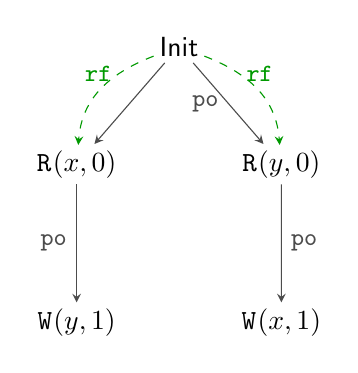
\begin{tikzpicture}[yscale=1,xscale=1.3]

        \node (init) at (1,  1.5) {$\Init$};

        \node (i11) at ( 0,  0) {$\rlab{}{x}{0}$};
        \node (i12) at ( 0, -2) {$\wlab{}{y}{1}$};

        \node (i21) at ( 2,  0) {$\rlab{}{y}{0}$};
        \node (i22) at ( 2, -2) {$\wlab{}{x}{1}$};

        \draw[po] (i11) edge node[left] {\small$\lPO$} (i12);
        \draw[po] (i21) edge node[right] {\small$\lPO$} (i22);

        \draw[po] (init) edge (i11);
        \draw[po] (init) edge node[left] {\small$\lPO$} (i21);

        \draw[rf] (init) edge[bend right] node[above] {\small$\lRF$} (i11);
        \draw[rf] (init) edge[bend left]  node[above] {\small$\lRF$} (i21);

      \end{tikzpicture}
    \end{minipage}
    \hfill
    \begin{minipage}[c][1\width]{0.3\textwidth}
      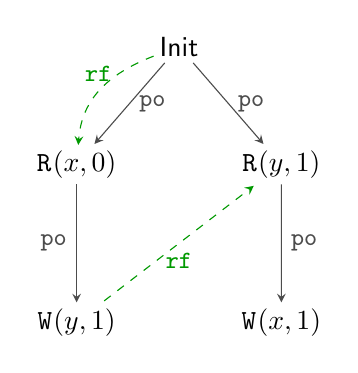
\begin{tikzpicture}[yscale=1,xscale=1.3]

        \node (init) at (1,  1.5) {$\Init$};

        \node (i11) at ( 0,  0) {$\rlab{}{x}{0}$};
        \node (i12) at ( 0, -2) {$\wlab{}{y}{1}$};

        \node (i21) at ( 2,  0) {$\rlab{}{y}{1}$};
        \node (i22) at ( 2, -2) {$\wlab{}{x}{1}$};

        \draw[po] (i11) edge node[left] {\small$\lPO$} (i12);
        \draw[po] (i21) edge node[right] {\small$\lPO$} (i22);

        \draw[po] (init) edge node[right] {\small$\lPO$} (i11);
        \draw[po] (init) edge node[right] {\small$\lPO$} (i21);

        \draw[rf] (init) edge[bend right] node[above] {\small$\lRF$} (i11);
        \draw[rf] (i12)  edge             node[below] {\small$\lRF$} (i21);

      \end{tikzpicture}
    \end{minipage}
    \hfill
    \begin{minipage}[c][1\width]{0.3\textwidth}
      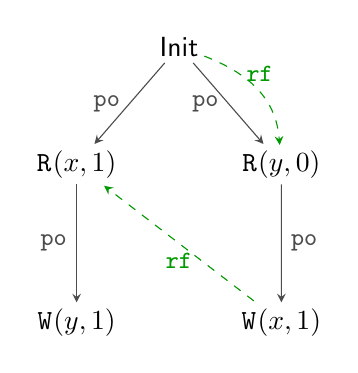
\begin{tikzpicture}[yscale=1,xscale=1.3]

        \node (init) at (1,  1.5) {$\Init$};

        \node (i11) at ( 0,  0) {$\rlab{}{x}{1}$};
        \node (i12) at ( 0, -2) {$\wlab{}{y}{1}$};

        \node (i21) at ( 2,  0) {$\rlab{}{y}{0}$};
        \node (i22) at ( 2, -2) {$\wlab{}{x}{1}$};

        \draw[po] (i11) edge node[left] {\small$\lPO$} (i12);
        \draw[po] (i21) edge node[right] {\small$\lPO$} (i22);

        \draw[po] (init) edge node[left] {\small$\lPO$} (i11);
        \draw[po] (init) edge node[left] {\small$\lPO$} (i21);

        \draw[rf] (i22)  edge             node[below] {\small$\lRF$} (i11);
        \draw[rf] (init) edge[bend left ] node[above] {\small$\lRF$} (i21);

      \end{tikzpicture}
    \end{minipage}
    \begin{minipage}[c][1\width]{0.3\textwidth}
      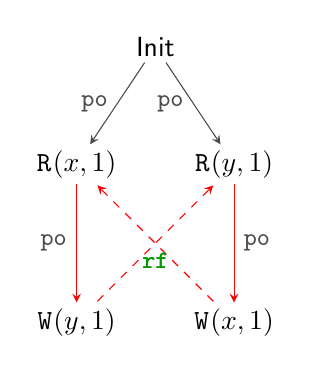
\begin{tikzpicture}
        \node (init) at (1,  1.5) {$\Init$};

        \node (i11) at ( 0,  0) {$\rlab{}{x}{1}$};
        \node (i12) at ( 0, -2) {$\wlab{}{y}{1}$};

        \node (i21) at ( 2,  0) {$\rlab{}{y}{1}$};
        \node (i22) at ( 2, -2) {$\wlab{}{x}{1}$};

        \draw[po, red] (i11) edge node[left] {\small$\lPO$} (i12);
        \draw[po, red] (i21) edge node[right] {\small$\lPO$} (i22);

        \draw[po] (init) edge node[left] {\small$\lPO$} (i11);
        \draw[po] (init) edge node[left] {\small$\lPO$} (i21);

        \draw[rf, red] (i22)  edge             node[below] {\small$\lRF$} (i11);
        \draw[rf, red] (i12)  edge             node[below] {\small$\lRF$} (i21);
      \end{tikzpicture}
    \end{minipage}
  \end{figure}

  Теперь, когда мы абстрагировались от кода программы, мы можем анализировать полученные из отношений
  графы. Например, так как последнее поведение нельзя воспроизвести поочередным исполнением команд из
  разных потоков, то мы можем захотеть запретить его \cite{rc11}.
  Это легко сделать, потребовав иррефлексивность транзитивного замыкания
  объединения отношений: $ (\textit{po} \cup \textit{rf})^+ $. 

  Такой анализ обычно преследует следующие цели:
  \begin{itemize}
    \item сформулировать ограничения на исполнения программы:
    например, модель памяти RC11 запрещает поведения, в которых отношение <<произошло до>> содержит
    циклы \cite{rc11}.
    \item доказать вложенность одной модели в другую:
    например, компиляция нашего языка под архитектуру POWER корректна, если после нее в модели
    архитектуры \cite{axiomatic_memory_model_for_power_mp} не появилось новых поведений относительно
    модели памяти языка.
    \item оценить свойства исполнения или модели в целом:
    например, монотонность модели, которая говорит о том, что если части исполнения программы
    допустимы, то и все исполнение допустимо.

  \end{itemize}

  Анализу также сопутствуют формальные доказательства всех утверждений и свойств, например, в системе Coq.
  И так как базовый формализм аксиоматических моделей памяти основан на бинарных отношениях, нам часто
  приходится доказывать свойства бинарных отношений, их равенства или неравенства, которые не
  специфичны для моделей памяти (универсальны) и могут быть автоматизированы.
  % TODO: Возможно тут слишком слаба обосновательная база для применения автоматизации

  Поэтому цель данной работы состоит в том, чтобы упростить доказательства в моделях памяти путем
  автоматизации доказательств свойств бинарных отношений.

  \section{Анализ Алгебры Клини и ее расширения}

    Бинарные отношения мы представим как алгебру с предикатами равенства ($ = $) и неравенства ($ \leq $),
    через которые впоследствии будем выражать все остальные их свойства.

    Определим формальную алгебру Клини, относительно которой бинарные отношения полны и корректны как модель.
    Это позволит нам с помощью проверки выводимости в алгебре Клини проверять равенства и неравенства бинарных отношений.

    Затем мы рассмотрим различные расширения алгебры Клини и проанализируем их полезность в контексте
    моделей памяти.

    В конце раздела можно найти краткие итоги этого анализа в виде
    \hyperref[tab:compare_algebras]{Таблицы \ref{tab:compare_algebras}}.

    \subsection{Алгебра отношений}
      Для некоторого множества $ O $, зададим \textit{бинарные отношения}
      $ a, b \subseteq \mathcal{P}(O \times O) $
      и операции над ними:
      \begin{itemize}
        \item композиция:
         $$a \cdot b \triangleq \{ (x, y) : \exists z : (x, z) \in a, (z, y) \in b \} $$
        с нейтральным элементом (множеством всех петлей) $ 1 \triangleq \{(x, x) : x \in O\} $
        и нулем (пустым отношением) $ 0 \triangleq \emptyset $
        \item рефлексивное транзитивное замыкания:
        $$ a^* \triangleq \bigcup\limits_{n \in \overline{0..n}} a^n $$,
       где
       \begin{equation*}
        a^n \triangleq \begin{cases}
          a^{n-1} \cdot a & n > 1\\
          1          & n = 0
        \end{cases}
       \end{equation*}
       \item объединение:
       $$ a \cup b = \{(x, y) : (x, y) \in a ~\text{или}~ (x, y) \in b   \} $$

      \end{itemize}
      Также будем пользоваться нотацией для транзитивного замыкания: $ x^+ \triangleq x \cdot x^*$.

      \textit{Алгеброй отношений} $\mathit{Rel}\langle O \rangle$
      назовем кортеж  $\langle O, \cup, \cdot, \_^* , 0, 1\rangle $.

      Для любых двух выражений $ f, e \in \mathit{Rel}$ определим выражение \textit{равенства} и
      \textit{неравенства}, как теоретико-множественные операции равенства и включения множеств
      соответственно:

      $$ f = e \triangleq f \subseteq e \wedge e \subseteq f \;\;\;\;\;\;\;\;\;\;\;\;\; f \leq e \triangleq f \subseteq e $$

      Обозначим за $\mathit{Rel}$ - класс алгебр $ \mathit{Rel}\langle O \rangle $ для всех $ O $.

      Для определения общезначимости оценки выражения введем еще несколько обозначений:
      \begin{itemize}
        \item конечный алфавит $ \Sigma $
        \item выражения $ f, e $ состоящие из конечного количества связок
        ($ \cup, \cdot, \_^* , 0, 1 $) и атомарных переменных из алфавита $ \Sigma $.
        \item элементарная функция оценки S, которая сопоставляет атомарным переменным некоторые
          бинарные отношения из алгебры $ R \langle O \rangle $.
      \end{itemize}
      Тогда (не)равенство выражений $ f $ и $ g $ является \textit{общезначимым в классе алгебр отношений}
      ($\mathit{Rel} \models f \leq g, \mathit{Rel} \models f = g $),
      если после оценки переменных любой функцией $ S $ для любой алгебры $ \mathit{Rel}\langle O \rangle $
      получается верное (не)равенство бинарных отношений.

    % TODO: возможно стоит убрать аксиомы
    \subsection{Алгебра Клини}
      % TODO: link на аксиоматизацию
      Назовем \textit{Алгеброй Клини} кортеж $\langle A,\cup,\cdot,\_^*,0,1\rangle$ такой, что $\langle A, \cup, \cdot, 0, 1 \rangle$ - идемпотентное полукольцо и операция $ \_^* $ удовлетворяет ряду аксиом:
      \begin{enumerate}
        \item $ 1 \cup a \cdot a^* \leq a^* $
        \item $ 1 \cup a^* \cdot a \leq a^* $
        \item $ b \cup a \cdot x \leq x \Rightarrow a^* \cdot b \leq x $
        \item $ b \cup x \cdot a \leq x \Rightarrow b \cdot a^* \leq x $
      \end{enumerate}
      где  $ a \leq b \triangleq a \cup b = b$

      Тогда за \textit{KA} обозначим аксиоматизированную теорию над алгеброй Клини, состоящую аксиом
      идемпотентного полу-кольца и аксиом (а-г).

      Записью $ \mathit{KA} \vdash f = g $ будем обозначать факт, что равенство $ f = g $, является
      логическим следствием аксиом \textit{KA}.
      Аналогично определим $ \mathit{KA} \vdash f \leq g $.

      Известно, что теория алгебры Клини разрешима и является PSpace-полной \cite{word_problem_pspace}.
      Также \textit{KA} полна и корректна относительно алгебры отношений \cite{AlgebrasOfRelation}: 
      $ \mathit{Rel} \models f = g $ $ \Leftrightarrow \mathit{KA} \vdash f = g$.

      Поэтому если мы формализуем в Coq процедуру разрешения \textit{KA}-(не)равенств, мы можем
      автоматически доказывать общезначимые факты для бинарных отношений, которые удовлетворяют
      сигнатуре \textit{Rel}.
      Существующие реализации будут рассмотрены ниже.

      Уже такой небольшой набор операций позволит нам сформулировать с помощью (не)равенств
      \textit{KA}-выражений, например, условие рефлексивности отношения $ r $:
      $$ r = r \cup 1 $$
      Пояснение: рефлексивное отношение содержит в себе все петли, то есть $ 1 $, поэтому при
      объединении не изменится.

      Или решать сложные неравенства, которые иногда возникают на практике:

      $$ (r_1 \cup r_2)^+ \leq r_1^+ \cup r_2^+ \cdot r_1^* \cup r_2^* \cdot (r_1^+ \cdot r_2^+)^+ \cdot r_1^* $$

    \subsection{Алгебра Клини с тестами}
      Теперь рассмотрим очень полезное расширение KA: алгебра Клини с тестами.

      \textit{Клини алгебра с тестами}, это кортеж $\langle K,\mathbb{B}, [\cdot] \rangle$ такой, что:

      \begin{itemize}
        \item $K$ - Клини алгебра $\langle A, \cup, \cdot, \_^*, 0, 1 \rangle $
        \item $\mathbb{B}$ - булева алгебра $\langle B, \wedge, \vee, \neg, \top, \bot \rangle $ (тесты)
        \item $[\:\_\:]$ - гомоморфизм из
          $\langle B, \vee, \wedge, \top, \bot \rangle$
        в $\langle A, \cup,  \cdot, 1, 0 \rangle$
      \end{itemize}
      % TODO надо ли сказать, что такое гомоморфизм?
      % TODO нужен ли линк на аксиоматизацию?
      Аналогично за $ \mathit{KAT} $ обозначим аксиоматическую теорию, состоящую из аксиом \textit{KA},
      аксиом булевой алгебры $ \mathbb{B}$ и свойств гомоморфизма.
      И аналогично обозначим за $ KAT \vdash f = g, f \leq g $ выводимость в этой теории.

      Также расширим определение бинарных отношений $Rel \langle O \rangle $, добавив булеву алгебру $\langle
      \mathcal{P}\langle O \rangle, \cap, \cup, O, \emptyset \rangle$ и гомоморфизм $ [a] \triangleq \{(x, x): x \in a\} $.
      То есть тесты в модели бинарных отношений - это множества элементов из $O$, которые можно
      воспринимать как логические элементы. А гомоморфизм $[\:\_\:]$ сопоставляет им множество петель.
      Последовательная композиция отношений с тестами позволяет фильтровать их истинностным значениям
      этих тестов.

      Такая расширенная алгебра отношений полна и корректна относительно алгебры Клини с тестами
      \cite{kat_completeness}: $\mathit{KAT} \vdash f = g \Leftrightarrow \mathit{Rel} \models f = g$.
      
      Задача разрешения (не)равенств в \textit{KAT} разрешима, является PSpace-полной
      \cite{kat_complexity} и существует формализация в Coq \cite{kat}, которая будут рассмотрены в
      следующих разделах.

      В моделях памяти доменами отношений являются элементарные события, потому данная теория позволяет
      нам накладывать любые вычислимые предикаты на события в программе. Например, мы можем определить
      множество операций чтения/записи как W/R соответственно.
      Это позволяет нам, сказать, что отношение <<прочитано из>> (rf) задано только между
      операциями чтения и записи \cite{rc11}:
      $$ \text{rf} \leq [W] \cdot \text{rf} \cdot [R] $$
      Пояснение: $ [W] $ - это множество петель над событиями записи, а $[R]$ - над операциями чтения.
      Если ребра отношения \textit{rf} существуют только между ними, то после фильтрации отношение не
      уменьшится. 

%     Это дает нам возможность выразить переход между фиксированными командами $ a $ и $ b $:
%    $ [\lambda x, x = a]\cdot 1 \cdot[\lambda x, x =b] $. Или например факт того, что если какое-то утверждение $ d $
%    верно в домене, то будет верно и на кодомене отношения можно выразить так: $ [!d] \cdot r \cdot [d] \leq 0 $

    \subsection{Алгебры Клини с инверсией}
      Теперь добавим к алгебре Клини операцию инвертирования $ \_^{\smile} $, удовлетворяющую следующим аксиомам:
      \begin{enumerate}
        \item $ (a \cup b)^{\smile} = a^{\smile} \cup b^{\smile} $
        \item $ (a \cdot b)^{\smile} = b^{\smile} \cdot a^{\smile} $
        \item $ (a^*)^{\smile} = (a^{\smile})^* $
        \item $ {a^{\smile}}^{\smile} = a $
        \item $ a \leq a \cdot a^{\smile} \cdot a $
      \end{enumerate}
      тогда мы получим теорию, так называемую \textit{Алгебрами Клини с инверсией} (\textit{KAC}).
      В ней аналогично с \textit{KA} определяются (не)равенства, оценки и выводимость.

      В алгебре отношений операции инвертирования соответствует операция переворачивания всех ребер:
      $$ a^\smile \triangleq \{ (y, x): (x, y) \in a \} $$

      \textit{KAC} корректна и полна относительно бинарных отношений с операцией инверсии, но не
      корректна относительно регулярных языков, в частности, аксиома (д) в них не выполнена. Теорию без
      этой аксиомы обычно обозначают как \textit{KAC}$^-$ \cite{AlgebrasOfRelation}.

      Для \textit{KAC} задача разрешимости остается PSpace-полной, но в сравнении с \textit{KAC}$^-$,
      алгоритмы разрешения пока что сложны для формализации в Coq \cite{AlgebrasOfRelation}, поэтому
      полных реализаций пока нет.

      В моделях памяти иногда возникают функциональные отношения, для которых верно, что каждому
      элементу слева отношение сопоставляет не более одного справа.
      Свойство, что отношение $ r $ является функциональным, можно выразить в
      \textit{KAC} с помощью операции инвертирования ($ \_^{\smile} $):
      $$ r^{\smile} \cdot r \leq 1 $$
      Пояснение: если отношение функциональное, то любой переход по ребру от <<значения>> к
      <<аргументу>> и по любому другому ребру опять к <<значению>> приведет нас в тоже значение. То
      есть композиция таких переходов - это всегда петля.

    \subsection{Решетки Клини}
      Теперь рассмотрим одно из самых значительных расширений алгебр Клини.
      Если мы добавим к \textit{KA} операцию пересечения($\cap$),
      то получим \textit{решетку Клини} (\textit{KL}).

      Алгебра отношение \textit{Rel} в этом случае дополняется следующей операцией:

      $$ f \cap e \triangleq \{ (x, y) \colon (x, y) \in f \wedge (x, y) \in e \} $$

      Данная аксиоматическая теория является разрешимой \cite{petri_for_kal}, но алгоритм разрешения чрезвычайно
      сложен и требует экспоненциального количества памяти, поэтому автоматизация (не)равенств из этой
      теории в Coq пока не представляется возможной. Также существует доказательство того, что
      эта задача является EXPSpace-полной задач \cite{complexity_of_regular_intersection}.
      
      Тем не менее операция пересечения была бы очень полезна в моделях памяти.
      Часто ограничение на исполнение программы формулируется как ацикличность отношения <<произошло
      до>>, которое в свою очередь является комбинацией других базовых отношений \cite{rc11}. С помощью
      новой операции ацикличность легко выразить неравенством:
      $$ r^+ \cap 1 \leq 0 $$
      Пояснение: любой цикл при транзитивном замыкании приводит к появлению петлей и наоборот.

    % NOTE: Зоопарк рано закрывался и мы не все успели посмотреть:
    %       GKAT, NetKAT,  Pointer KA, Concurrent KA, Nominal KA, KA with relation, Mutable tests

    \subsection{Аллегории Клини}
      Если же мы одновременно добавим в алгебру Клини операции пересечения $\cap$ и инверсии ($\_^{\smile}$),
      то получим богатую теорию \textit{аллегорий Клини (KAl)}.

      Недавние результаты показывают, что для такой теории существует система аксиом, которая полна и
      корректна для бинарных отношений \cite{axioms_kal} (с доказательством на Coq). Она также разрешима
      и EXPSpace-полная \cite{dec_kal}.

      При этом еще остаются открытые вопросы, например, о возможности добавлении в теорию универсального
      отношения ($\top \triangleq O \times O $) \cite{axioms_kal}.
      % TODO: поддерживает ли эта аксиоматизация тесты?
      
    \begin{table}[!h]
      \caption{Сравнение расширений алгебр Клини}
      \label{tab:compare_algebras}
      \centering
      \begin{tabularx}{\textwidth}{|*{18}{>{\centering\arraybackslash}X|}}\hline
        Название & Пример доказываемого свойства & Сложность & Реализация в Coq
        \\\hline
        \textit{KA} & Рефлексивность, Транзитивность & PSpace & relation-algebra, atbr
        \\\hline
        \textit{KAT} & Предикаты на доменах & PSpace & relation-algebra
        \\\hline
        \textit{KAC} & Функциональные отношения & PSpace &
        \\\hline
        \textit{KL}  & Ацикличность, Разность & EXPSpace &
        \\\hline
        \textit{KAl} & \textit{KAC} + \textit{KL} & EXPSpace &
        \\\hline
      \end{tabularx}
    \end{table}

  \section{Анализ существующих реализаций в Coq}\label{section:coq_impls}
    % NOTE - Что требуется для достижения цели
    %      - Что уже сделано
    %      - Почему сделанного недостаточно

    Теперь рассмотрим существующие реализации алгебры Клини и ее расширений в Coq: библиотеки
    atbr \cite{atbr} и relation-algebra \cite{kat}.
    Остановимся на каждой подробно и опишем их минусы и плюсы.
    % NOTE: Есть еще реализация \cite{moreira}, которая вроде по-другому формализует решалку и работает
    % иногда на порядок быстрее atbr. Но я не нашел к у них исходников. Видимо их нет в публичном доступе

    \subsection{abtr}

      Эта библиотека предоставляет инструменты для автоматического доказательства общезначимых
      (не)равенств в \textit{KA} и \textit{KAC}$^-$.

      То есть операция инверсии ($\_^\smile$) не работает во всех случаях для бинарных отношений. Это лишает
      нас гарантии, что общезначимое (не)равенство, содержащее эту операцию, будет доказано
      автоматически. Алгоритм разрешения \textit{KAC}$^-$ значительно проще, чем для \textit{KAC} и
      вряд ли может быть полезен для бинарных отношений.
      
      \textit{KA} реализована в полной мере с доказательством теоремы о полноте, что позволяет быть
      уверенным в корректности кода библиотеки.

    \subsection{relation-algebra}

      Эта библиотека является развитием atbr, в которой допущена ошибка при дизайне, и поэтому
      авторам перед расширением функционала пришлось переписать ее с нуля. В ней реализована полная
      поддержка \textit{KAT} и \textit{KA}.

      Также важно отметить, что relation-algebra реализует алгоритм исключения гипотез
      \cite{hkat, hkat_cpc}, что позволяет автоматически доказывать
      не только общезначимые, но и те (не)равенства которые следуют из гипотез определенного вида, а
      конкретнее, сводящиеся к равенствам Хоара ($ r = 0 $).
      % TODO: <<равенства>> Хоара - это какой-то не очень устоявщийся термин

      Это чрезвычайно полезно на практике.
      Например, мы можем доказывать монотонность некоторых свойств отношений,
      то есть если факт того, что если для нескольких отношений свойство выполняется, то и для их
      комбинации оно тоже будет выполнено.
      К примеру монотонность пустоты отношений:
      $$ r_1 \leq 0, r_2 \leq 0 \vdash (r_1 \cdot r_2) \leq 0 \;\;\;\;\;\;\;\;\;\;\;\;\; r \leq 0 \vdash r^+ \leq 0 $$

      В своем интерфейсе библиотека использует канонические структуры и классы типов
      \cite{canonical_structures} в качестве средств полиморфизма. Это позволяет обобщить алгоритм
      разрешения (не)равенств для любой структуры, которая отвечает сигнатуре и аксиомам \textit{KAT}.
      
      Чтобы генерация доказательств работала для конкретно заданной структуры необходимо предъявить
      операции, соответствующие сигнатуре \textit{KAT} и доказать, что для них выполнены все аксиомы.

\finishrelatedwork

  \section{Постановка задачи}
    % NOTE Текст здесь должен следовать из цели (см. введение)
    % NOTE Следующая глава должна ссылкать на эти задачи и показывать, почему они решены

    % TODO Возможно формулировка того, где мы применяем KAT надо обобщить ?

    Для того, чтобы исследовать применение теории алгебры Клини на практике, была взята библиотека hahn \cite{hahn}.
    Она содержит базовую формализацию модели исполнения и доказательства огромного числа лемм, которые
    непосредственно используются для построения различных моделей памяти \cite{imm}.

    % TODO: Может быть стоит уточнить задачи: аксиомы, переформулирование, применение.
    Так как цель этой работы заключается в исследовании применимости теории Клини к моделям памяти,
    то задача этой работы состоит в оценке объема доказательств в hahn, которые возможно упростить с помощью relation-algebra.


  \chapterconclusion
    Расширения алгебры Клини способны сильно облегчить работу с аксиоматическими моделями памяти,
    так как через них можно выразить многие важные в этой области свойства. К сожалению, немногие
    расширения возможно реализовать в Coq эффективно и даже те, что реализованы, потребовали огромного труда разработчиков.

    Тем не менее, возможно уже текущие разработки в этой области могут существенно упростить работу с моделями памяти.

\chapter{Применение \textit{KAT} к моделям памяти}\label{chapter:2}
 % Needs:
 % TODO Предполагаемое теоретическое решение
 % TODO Обоснование, почему оно удовлетворяет требованиям, сформулированным в первой главе
 % TODO Теоретическое сравнение с существующими решениями

  Теперь опишем предлагаемый способ применения библиотеки для автоматического разрешения (не)равенств
  бинарных отношений с тестами relation-algebra для упрощения доказательств в библиотеке hahn.

  Далее сравним новый подход к автоматизации доказательств с теми, которые уже применяются в hahn для автоматизации доказательств.

  \section{Описание решения проблемы}

    В Coq доказательства состоят из последовательности команд (\textit{тактик}), каждая из
    которых упрощает или полностью доказывает текущее утверждение.

    Библиотека relation-algebra предоставляет тактики \coqe{kat} и \coqe{hkat},
    которые позволяют автоматически доказать общезначимые или следующие из специальных гипотез
    (не)равенства соответственно.

    Как упоминалось в первой главе, для их использования необходимо определить сигнатуру \textit{KAT} для
    используемой в hahn реализации бинарных отношений и доказать выполнимость аксиом.

    Чтобы автоматически доказать с помощью новых тактик какое-то утверждение необходимо, чтобы оно было
    сформулировано как проверка общезначимости \textit{KAT}-(не)равенств (или как проверка следствия из
    гипотез, с которыми способна работать \coqe{hkat}).
    Поэтому также необходимо переформулировать некоторые утверждения.

    \subsection{Определение экземпляра \textit{KAT}}

      В библиотеке hahn уже определены многие базовые операции с бинарными отношениями, такие как
      объединение ($r_1 \cup r_2$) или композиция ($r_1 \cdot r_2$). Поэтому предлагается
      лишь объявить экземпляр канонической структуры \coqe{kat.ops}, который сопоставляет сигнатуру
      \textit{KAT} с уже определенными операциями.
      Также этот экземпляр содержит булеву алгебру доменов отношений, которая была для этого мной
      объявлена.

      Далее интерфейс библиотеки relation-algebra требует определить экземпляр класса типа
      \coqe{kat.laws}, содержащий доказательства выполнения всех аксиом \textit{KAT} для наших операций.
      Все они были доказаны с помощью встроенных в Coq тактик, а также частично были переиспользованы
      леммы из relation-algebra.

      После этого механизмы вывода типов в Coq могут восстановить информацию о том, что выражение
      принадлежит \textit{KAT}-сигнатуре, если оно состоит из соответствующих операций.
      Поэтому тактики \coqe{kat(hkat)} смогут автоматически сгенерировать доказательства для
      утверждений, если те являются
      общезначимыми (или следуют из специальных гипотез).

      % TODO: выбивается из рассказа и не понятно нужно ли оно вообще здесь
      % Например, в библиотеке уже имеется доказательства того, что встроенный в Coq тип утверждений Prop отвечает
      % аксиомам булевой алгебры, а также лемму о том, что мы можем поточечно расширять алгебраическую структуру.
      % Применив эту лемму к булевой алгебре Prop, мы получим булеву алгебру предикатов $ A \rightarrow Prop $. А применив
      % второй раз, мы получим как раз определения бинарных отношений в hahn $ A \rightarrow A \rightarrow Prop $.

    \subsection{Переформулирование определений}

      Некоторые леммы в hahn сформулированы в терминах не принадлежащих сигнатуре \textit{KAT}, но тем не менее
      могут быть в ней сформулированы.

      Для примера рассмотрим утверждение \coqe{max_elt a r}.
      Оно означает, что \coqe{a} является максимальным событием в отношении \coqe{r}, то есть из \coqe{a} нет исходящих
      ребер отношения. В hahn оно определяется так:

      \begin{lstlisting}[gobble=8]
        Definition max_elt {A: Type} (r: relation A) (a: A) :=
          forall (b: A), not (r a b).
      \end{lstlisting}

      Оно не отвечает сигнатуре алгебры Клини с тестами, и его нельзя доказать автоматически.
      Но его можно переформулировать так $ [eq\ a] \cdot r \le \emptyset $, где $eq\ a$ - предикат проверяющих событие на равенство
      c $a$.
      То есть $ a $ - максимальный элемент тогда и только тогда, когда множество путей, которые сначала
      проходят по петле в элементах равным $a$, а потом по отношению r, пусто (из $a$ есть исходящий переход).

      Чтобы формально обосновать предположение о том, что оба этих определения эквиваленты, докажем лемму:
      \begin{lstlisting}[gobble=8]
        Lemma max_elt_iff_kat:
          forall (a: A) (r: relation A), max_elt r a <-> [eq a] \cdot r \leq \emptyset.
      \end{lstlisting}
        % Proof.
        %   unfold_all; unfold max_elt; firstorder.
        %   - eapply H. rewrite H2, H0. apply H1.
        %   - eapply H. esplits; eauto.
        % Qed.

      Также, используя эту лемму, с помощью последовательного применения встроенной тактики
      \coqe{rewrite} мы можем в процессе доказательства заменять старые определения на новые: 

      \begin{lstlisting}[gobble=8]
        Lemma max_elt_iter: max_elt r a -> max_elt r^+ a.
        Proof.
          repeat rewrite -> max_elt_iff_kat.
          (* current goal: [eq b] \cdot r \leq \emptyset -> [eq b] \cdot r^+ \leq \emptyset *)
          hkat.
        Qed.
      \end{lstlisting}

      Если утверждение примет необходимый вид, то \coqe{(h)kat} автоматически докажет его.
      
      Благодаря такому подходу мы не будем переписывать определения всех теорем и лемм, а только изменим их доказательства.
      Это сохранит их интерфейс и не сломает нетронутых доказательств, которые используют переформулируемые утверждения.

      В этом примере у нас получилось привести исходное определение \coqe{max_elt} к виду $r \leq \emptyset$, что
      дает возможность автоматически доказывать утверждения вида \coqe{max_elt a r}, но и использовать
      их в качестве гипотез.
      Благодаря этому, после переписывания всех вхождений \coqe{max_elt} в утверждении леммы
      \coqe{max_elt_iter}, тактика \coqe{hkat} автоматически сгенерировала остальное доказательство.

      Кроме гипотез вида $r \leq \emptyset$ библиотека relation-algebra поддерживает гипотезы нескольких других
      видов \cite{kat}, которые к нему сводятся или могут быть исключены \cite{hkat,hkat_cpc}:
      \begin{itemize}
        \item $ r = 0 $
        \item $[a] \cdot x = x \cdot [b]$, $[a] \cdot x \leq x \cdot [b]$
        \item $x \cdot [a] = [b] \cdot x$, $x \cdot [a] \leq [b] \cdot x$
        \item $ r \leq [a] \cdot r $, $ r \leq r \cdot [a]$
        \item $ a = b $, $ a \leq b $
        \item $[a] \cdot r = [a]$, $r \cdot [a] = [a]$, где $r$ - атомарная переменная
      \end{itemize}

      Исходя из выше описанного, все определения в hahn, которые получилось выразить в сигнатуре
      \textit{KAT} разделить на 3 группы:
      \begin{enumerate}
        \item утверждения, которые можно использовать как гипотезы и доказывать их автоматически
        \item утверждения, которые нельзя использовать как гипотезы, но можно их доказывать
        \item определения отношений, которые могут входить утверждения первого или второго типа.
      \end{enumerate}

      В \hyperref[tab:redefine_succ]{таблице \ref{tab:redefine_succ}} указаны все переопределения,
      которые удалось выполнить в hahn, разбитые по этим группам.
      Также в \hyperref[tab:redefine_fail]{таблице \ref{tab:redefine_fail}} можно найти несколько
      важных определений, которые не удалось выразить через \textit{KAT},
      но удалось через другие расширения алгебры Клини.

      \begin{table}[!h]
        \caption{Переформулирование определений в сигнатуру \textit{KAT}}
        \label{tab:redefine_succ}
        \centering
        \begin{tabularx}{\textwidth}{|*{18}{>{\centering\arraybackslash}X|}}\hline
          Название & Оригинальное определение & \textit{KAT}
          \\\hline
          \multicolumn{3}{|c|}{Переформулирование определений отношений}
          \\\hline

          $ restr\_rel\ p\ r $ & $ r\ x\ y \wedge p\ x \wedge p\ y $ & $ [p] \cdot r \cdot [p] $
          \\\hline
          $ clos\_refl\ r $ & $ x = y \wedge r\ x\ y $ & $ 1 \sqcup r $
          \\\hline

          \multicolumn{3}{|>{\centering\hsize=3\hsize}X|}
            {Переформулирование утверждений, которые можно использовать в качестве гипотез}
          \\\hline

          $ upward\_closed\ r\ p $ & $ \forall x y, r\ x\ y \rightarrow p\ y \rightarrow p\ x $ & $ r \cdot [p] \leq [p] \cdot r $
          \\\hline

          $ doma\ r\ p $ & $ \forall x y, r\ x\ y \rightarrow p\ x $ & $ r \leq [p] \cdot r $
          \\\hline
          $ domb\ r\ p $ & $ \forall x y, r\ x\ y \rightarrow p\ y $ & $ r \leq r \cdot [p] $
          \\\hline

          $ max\_elt\ a\ r $ & $ \forall b, \neg (r\ a\ b)$ & $ [eq\ a] \cdot r \leq 0 $
          \\\hline
          $ min\_elt\ a\ r $ & $ \forall b, \neg (r\ b\ a)$ & $ r \cdot  [eq\ a] \leq 0$
          \\\hline
          $ wmax\_elt\ a\ r $ & $ \forall b, r\ a\ b \rightarrow a = b $ & $ [eq\ a] \cdot r \leq [eq\ a] \cdot r \cdot
          [eq\ a] $
          \\\hline
          $ wmin\_elt\ a\ r $ & $ \forall b, r\ b\ a \rightarrow a = b $ & $ r \cdot [eq\ a] \leq [eq\ a] \cdot r \cdot [eq\ a] $
          \\\hline

          \multicolumn{3}{|>{\centering\hsize=3\hsize}X|}
            {Переформулированные утверждений, которые нельзя использовать в качестве гипотез}
          \\\hline

          $ transitive\ r $ & $ \forall x y z, r\ x\ z \!\rightarrow\! r\ z\ y \!\rightarrow\! r\ x\ y $ & $ r \cdot r \leq r $
          \\\hline
          $ reflexive\ r $ & $ \forall x, r\ x $ & $ 1 \leq r $
          \\\hline

          $dom\ b\ r$ & $ \forall x y, r\ x\ y \rightarrow x = b $ & $ r \leq [eq\ b] \cdot r$
          \\\hline
          $cod\ b\ r$ & $ \forall x y, r\ x\ y \rightarrow y = b $ & $ r \leq r \cdot [eq\ b]$
          \\\hline
        \end{tabularx}
        где
        \coqe{(eq a : A -> Prop)} - предикат равенства с \coqe{a},
        \coqe{(r : relation A)} - отношение,
        \coqe{(a, b : A)} - события,
        \coqe{(p, p$_1$, p$_2$ : A -> Prop)} - предикаты на событиях,
        \coqe{A} - тип доменов отношений, событий
      \end{table}

    % TODO: fix indent
    \begin{table}[!h]
      \caption{Переформулирование определений, которые не удалось выразить в KAT, но можно выразить в
        других расширениях алгебры Клини}
      \label{tab:redefine_fail}
      \centering
      \begin{tabularx}{\textwidth}{|*{18}{>{\centering\arraybackslash}X|}}\hline
        Название & Оригинальное определение & Новое определение
        \\\hline
        % $ minus\_rel\ r_1\ r_2 $ & $ r_1 \setminus r_2 $ & $ r_1 \mathbin{\textcolor{red}{\cap}}r_2\mathbin{\textcolor{red}{\neg}} $
        % \\\hline

        $ irreflexive\ r $ & $ \forall x, \neg (r\ x\ x) $ & $ 1 \mathbin{\textcolor{red}{\cap}} r \leq 0 $
        \\\hline

        $ acyclic\ r $ & $ irreflexive\ r^+ $ & $ 1 \mathbin{\textcolor{red}{\cap}} r^+ \leq 0 $
        \\\hline

        $ immediate\ r $ & $\! r\ a\ b \wedge (\forall c, r\ a\ c \!\rightarrow\! \neg (r\ c\ b)) $ & $ r \mathbin{\textcolor{red}{\cap}} 1 $
        \\\hline

        $ is\_total\ r $ & $\forall x y, r\ x\ y \vee r\ y\ x$ & $ r \cup r\mathbin{\textcolor{red}{^\smile}} \leq \mathbin{\textcolor{red}{\top}}$
        \\\hline

        $ cross\_rel\ p_1\ p_2 $ & $ p_1\ x \wedge p_2\ y $ & $ [p_1] \cdot \mathbin{\textcolor{red}\top} \cdot [p_2] $
        \\\hline

        $ singl\_rel\ a\ b $ & $ x = a \wedge y = b $ & $ [eq\ a] \cdot  \mathbin{\textcolor{red}\top} \cdot [eq\ b] $
        \\\hline

      \end{tabularx}
      Пояснение: \textcolor{red}{красным} выделены не выходящие в сигнатуру KAT связки,\\
      где $\top$ - универсальное отношение
    \end{table}

    Написав предложенные переопределения и доказав соответствующие леммы об их корректности, мы сможем
    автоматически доказывать утверждения, которые удалось выразить с помощью
    алгебры Клини с тестами, если они общезначимы или следуют из утверждений, которые удалось
    переформулировать в специальной форме.

      Важно отметить, что общезначимость означает, что для алгоритма разрешения (не)равенств предикаты
      непрозрачны. То есть он не может использовать свойства предикатов, которые следуют из их определения.

      Например, лемму \coqe{seq_eq_wmax} на \hyperref[lst:fail_eq]{Листинге \ref{lst:fail_eq}},
      \coqe{hkat} доказать не сможет, несмотря на то, что она принадлежащих сигнатуре \textit{KAT}, так
      как рассматривает \coqe{eq b} как атомарный символ.

      Но зная, что этот предикат \coqe{eq} выражает равенство, мы можем легко доказать свойство
      недостающее свойство (\coqe{[eq b] \cdot r \cdot [eq b] \leq [eq b]})
      и закончить доказательство леммы. К сожалению, это свойство нельзя использовать как гипотезу.
      \begin{lstlisting}[float=!h, gobble=6,
        caption={Пример не возможного использования hkat из-за нехватки гипотезы о внутреннем устройстве
        предиката}, label={lst:fail_eq}]
      Lemma seq_eq_wmax: wmax r b -> [eq b] \cdot r \leq [eq b].
      Proof.
        rewrite -> wmax_elt_iff_kat.
        (* current goal:
           [eq b] \cdot r \leq [eq b] \cdot r \cdot [eq b] -> [eq b] \cdot r \leq [eq b] *)
        Fail hkat. (* cann't solve *)
        assert ([eq b] \cdot r \cdot [eq b] \leq [eq b]) as H.
        { unfold_all; firstorder; congruence. }
        rewrite -> H; trivial
      Qed.
      \end{lstlisting}

      В заключении, чтобы удобно переписывать утверждения состоящие из разных определений, воспользуемся
      тактикой \coqe{autorewrite} \cite{coq_man}, что позволит использовать динамическую базу
      утверждений для переписывания, которую можно пополнять по мере добавления новых определений.
    
      Так же для удобства объявим тактики \coqe{(h)kat'}, которые будут применять \coqe{autorewrite},
      а потом вызывать \coqe{(h)kat'}, что также скроет все переформулировки от ее
      пользователя (см. \hyperref[lst:define_lift]{Листинг \ref{lst:define_lift}})

    % TODO: fix floating
      \begin{lstlisting}[float=false, gobble=4,
        caption={Переопределение тактик \coqe{h(kat)}, для автоматической замены старых определений на новые}, label={lst:define_lift}]
      Hint Rewrite restr_rel_iff_kat: redefDb.
      Hint Rewrite wmax_elt_iff_kat: redefDb.
      ...
      Ltac lift_to_kat_all := repeat autorewrite with redefDb in *.
      Ltac kat'  := lift_to_kat; kat.
      Ltac hkat' := ligt_to_kat; hkat.
      \end{lstlisting}

  \section{Сравнение с существующими решениями}

    На данный момент в hahn большинство доказательств состоит из ручного использования других, уже
    доказанных утверждений, их автоматического перебора и стандартных тактик Coq.

    Проблема ручного использования очевидна. И по крайней мере от части такого труда \coqe{(h)kat'}
    может помочь избавится.

    Автоматический же перебор тоже хорошо справляется с этой задачей, но он предназначен в первую
    очередь для простых утверждений. Проблема этого подхода заключается в том, что не всегда можно по
    утверждению понять <<простое>> ли оно. Иногда перебор занимает значительное
    времени и приходится параметризовать его глубиной перебора и вручную стараться выбирать
    минимальное возможное ее значение. Это делает использование этого подхода не удобным.

    Главным преимуществом использования автоматических средств доказательств утверждений из некоторой
    разрешимой теории заключается в том, что существует четкий критерий когда метод работает, а когда
    нет: если утверждение имеет сигнатуру этой теории и оно общезначимо в ней. Это не только делает его
    более удобным, но дает возможность формально доказывать корректность алгоритма генерации доказательств.

    Кроме предложенного метода к там средствам относятся, например, встроенная тактика \coqe{tauto}
    \cite{coq_man} для интуиционистского исчисления высказываний.

    Это помогает не только при выборе того или иного метода доказательства, но также дает целую область
    знаний о базовом формализме, на которую мы можем опереться в своих рассуждениях. Например, зная, что
    мы можем легко доказать любое свойство бинарных отношении с тестами, разработчик может выписать через
    (не)равенство необходимое преобразование текущего утверждения, доказать его одной тактикой
    \coqe{(h)kat} и выполнить преобразование:

    \begin{lstlisting}[float=false, gobble=4,
      caption={Пример доказательства вспомогательного утверждения, необходимого для преобразования, с
        помощью \textit{KAT}}, label={lst:arewrite}]
    Proof.
    ...
    (* current goal: irreflexive (dd^* \cdot (dd^* \cdot de \cdot ee^* \cdot ed)^+) *)
    assert (dd^* \cdot (dd^* \cdot de \cdot ee^* \cdot ed)^+ \leq (dd^* \cdot de \cdot ee^* \cdot ed)^+) as H.
    { kat'. }
    rewrite -> H.
    (* current goal: irreflexive ((dd^* \cdot de \cdot ee^* \cdot ed) ^+) *)
    ...
    Qed.
    \end{lstlisting}

    Все же автоматический перебор покрывает большее число простых случаев, потому что слабо ограничен сигнатурой.
    Но, например, даже самое простое утверждение, которое содержит пересечение отношений, \coqe{(h)kat}
    решить не в силах. Но по мере усложнения утверждений количество бесполезных действий совершаемых перебором резко
    увеличивается, чего не происходит с более специализированными методами.
    
    Поэтому эти два подхода дополняют друг друга.

  \chapterconclusion
    Применение \textit{KAT} для автоматизации доказательств - это не универсальный, но удобный
    инструмент, который служит дополнением к уже имеющимся, что может сделать  разработку моделей
    памяти проще и быстрее.
    % TODO: может еще че написать.

\chapter{Результаты}\label{chapter:3}
  % NOTE: описание, как результаты, полученные во второй главе реализуются на практике
  %       описание сложностей, с которыми столкнулись при реализации

  Теперь, когда мы получили возможность использовать новый метод автогенерации доказательств, проанализируем его
  применение к доказательствам в библиотеке hahn.

  Сначала мы рассмотрим проблемы, с которыми пришлось столкнуться при этом, и опишем как удалось полностью или
  частично их решить.

  После этого подробно будет описано как с помощью нового метода изменились доказательства в hahn.

  \section{Проблемы в использовании \coqe{(h)kat}}
    После реализации всех экземпляров классов типов и канонических структур оказалось, что Coq все еще
    не может восстановить информацию о том, что некоторые операции принадлежат сигнатуре \textit{KAT}.

    Так же оказалось, что тактика \coqe{hkat} тратит очень много времени на анализ гипотез, которая она
    может использовать для генерации доказательства.
    \subsection{Проблемы с выводом типов}
      Изначально библиотека была спроектирована с использованием наиболее общих интерфейсов. Поэтому
      сигнатура моноида, которую включает в себя \textit{KAT}, сформулирована с учетом
      поддержки гетерогенных структур.
      Применительно к бинарным отношениями это значит, что типы левых и правых концов могут
      отличаться.

      В hahn бинарные отношения гомогенные, то есть соединяются элементы одного и того же
      типа: типа событий в программе. Поэтому типы левых и правых концов, которыми
      параметризован моноид, не
      используются при определении экземпляра сигнатуры. В результате чего, механизм унификации Coq не
      может вывести эти типы, и тактики \coqe{kat} и \coqe{hkat} не работают.

      Решением этой проблемы стало явное указание типов-параметров моноида. Для этого определение
      тактик \coqe{kat} и \coqe{hkat} было скопировано и явно прописаны типы параметров. Заметим, что
      скопирована была не вся реализация этих тактик, а лишь верхний уровень, который вызывал
      алгоритм непосредственно разрешения (не)равенств. Этого оказалось достаточно.
      %TODO: ссылка сюда из места где мы говорим про определение (h)kat'

    \subsection{Скорость агрегации гипотез}

      Тактика \coqe{hkat} включает в себя алгоритм исключения гипотез \cite{hkat,hkat_cpc}, который
      сводит задачу доказательства из гипотез к доказательству общезначимого утверждения,
      и потом фактически применяет тактику \coqe{kat}. Этот алгоритм должен сначала агрегировать
      гипотезы, то есть привести их к одной гипотезе вида
      $r \leq 0$ и именно этот процесс занимает наибольшее время работы \coqe{hkat}, иногда больше минуты.

      Дело в том, что агрегация работает путем перебора всех текущих гипотез и последовательных попыток
      применения всех лемм агрегации, которые разбивают равенства на два неравенства, объединяют
      неравенства и приводят гипотезы из специального вида к $r \leq 0$.

      Главным образом проблема производительности была решена тем, что \coqe{hkat} была разделена на
      легкую (\coqe{hkat'}) и полную (\coqe{hkat''}) версии.
      В первой были оставлены только быстрые преобразования и объединение гипотез в одну.
      Это позволило ей почти всегда работать очень быстро.

      Чтобы легкая версия работала в большем числе случаев все переформулирования определений
      делались из расчета на то, что она может работать с ними.

      Полная же версия включает все прежние преобразования и используется редко (5\% случаев, см раздел
      статистика, TODO).

      Также было обнаружено, что перебор в агрегации был не эффективным, так как часто пытался
      трансформировать гипотезы, которые уже были приведены к виду $r \le 0$, что всегда оканчивалось
      неудачей. Поэтому разделением его на фазы удалось ускорить полную версию \coqe{hkat} в среднем на
      5-8 секунд на примерах из hahn.

      % TODO: Попробовать удалять все гипотезы перед запуском hkat, см HahnKat.v

  \section{Описание результатов}

    Некоторые доказательства в hahn получилось полностью автоматизировать, а некоторые значительно
    упростить. Рассмотрим отдельно каждую из этих групп доказательств, и в конце приведем полную
    статистику.

    \subsection{Примеры полностью доказанных утверждений}

      Доказательства, которые получилось полностью доказать с помощью новых тактик особенно интересны
      потому, что часто в них пропадает необходимость. Так получается из-за того, что те свойства,
      которые они выражают уже <<содержатся>> в новом инструменте и могут быть полностью заменены им.

      Как и было предсказано в главе два полностью автоматизировались доказательства утверждений
      состоящих из свойств, которые \coqe{hkat} может использовать как гипотезы
      (см. \hyperref[tab:redefine_succ]{Таблицу \ref{tab:redefine_succ}}).

      Например монотонность свойства элемента быть максимальным в отношении:
      \begin{lstlisting}[float=false, gobble=8]
        Lemma max_elt_t : max_elt r a -> max_elt (r^+) a.
        Proof.
          (* red; ins; apply clos_trans_t1n in REL; induction REL; eauto. *)
          hkat'.
        Qed.
      \end{lstlisting}

      % TODO: Не уверен в плавности этого перехода.
      Также сильно упростилась работа с преобразованиями отношений.
      Например, чтобы, исходя из некоторых гипотез, доказать ацикличность объединения
      отношений ($r \cup r'$), она сначала сводится к иррефлексивности транзитивного замыкания
      $(r \cup r')^+$.
      Затем необходимо заменить это отношения на его надмножество $r^+ \cup (r^* \cdot r')^+ \cdot r^+$.
      Факт того, что это действительно надмножество и такое преобразование
      верно, вынесен в отдельную лемму \coqe{path_union} (\hyperref[lst:path_union_before]{Листинг \ref{lst:path_union_before}})
      с нетривиальным доказательством, которое использовало перебор с разной глубиной
      (\coqe{basic_solver n}).

      Сейчас доказательство леммы полностью автоматизированно (см.
      \hyperref[lst:path_union_after]{Листинг \ref{lst:path_union_after}}).

      \begin{lstlisting}[float=false, gobble=8, label={lst:path_union_before},
        caption={Пример сложного доказательства, которое может быть полностью автоматизированно}]
        Lemma path_union (r r': relation A) :
          (r \cup r')^+ \leq r^+ \cup (r^* \cdot r')^+ \cdot r^+.
        Proof.
          apply inclusion_t_ind_right.
          unionL; [vauto|].
          by rewrite rtE; rewrite <- !ct_step; basic_solver 12.
          relsf; unionL.
          - by unionR left; rewrite ct_unit.
          - by rewrite !seqA; rewrite <- ct_end; basic_solver 12.
          - rewrite (ct_step (r^+ \cdot r')).
          rewrite <- inclusion_t_rt at 1; basic_solver 22.
          - rewrite !seqA, inclusion_t_rt at 1.
          rewrite <- (ct_end (r^* \cdot r')); basic_solver 12.
        Qed.
      \end{lstlisting}

      \begin{lstlisting}[float=false, gobble=8, label={lst:path_union_after},
        caption={Пример полностью автоматизированного доказательства}]
        Lemma path_union (r r': relation A) :
          (r \cup r')^+ \leq r^+ \cup (r^* \cdot r')^+ \cdot r^+.
        Proof. kat'. Qed.
      \end{lstlisting}

    \subsection{Примеры частичного применения \coqe{(h)kat}}
      Некоторые из тех доказательства, которые не удалось автоматизировать полностью, получилось
      значительно упростить.

      В таких доказательствах часто автоматизации мешает всего одна <<сложная>> гипотеза,
      и после ее использования оставшаяся часть доказательства решается автоматически. В некоторых
      случаях это позволяло сократить до 40 строк доказательства.

      Также иногда плодотворным является эвристический подход к исключению таких гипотез.
      К примеру, утверждение (\coqe{dom r b}) о том, что отношение \coqe{r} всегда начинается в
      событии, равном \coqe{b}, можно выразить в \textit{KAT} (\coqe{r = [eq b] \cdot r}), но нельзя
      использовать как гипотезу.

      Если это единственная гипотеза, которую мы не можем использовать, то мы можем попробовать
      заменить все вхождения \coqe{r} на
      \coqe{[eq b] \cdot r} и применить \coqe{hkat}. Для удобства можно определить тактику \coqe{elim_dom},
      которая делает переопределяет гипотезу и делает замену.

      \begin{lstlisting}[float=false, gobble=8, label={lst:dom}]
        Ltac elim_dom DOM :=
          apply dom_to_kat in DOM;
          rewrite DOM in *;
          clear DOM.

        Lemma seq_min_rt r r' b (MAX: min_elt r b) (DOM: cod b r'):
          r^* \cdot r' = r'.
        Proof.
          elim_dom DOM.
          (* current goal: r^* \cdot [eq b] \cdot r' = [eq b] \cdot r' *)
          hkat'.
        Qed.
      \end{lstlisting}

    \subsection{Общая статистика}

      В общем в hahn с помощью нового метода удалось сократить доказательства на 471 сточку, упростились
      доказательства более 150 теорем/лемм.
      Подробную статистику по каждой тактике можно посмотреть в
      \hyperref[tab:stats]{Таблице \ref{tab:stats}}.

      % При подсчете статистики использовались утилиты git diff и coqwc

      \begin{table}[!h]
        \centering
        \begin{tabularx}{\textwidth}{|*{18}{>{\centering\arraybackslash}X|}}\hline
          Тактика & Полностью доказанные леммы &
          Частично доказанные леммы & Количество строк сокращено 
          \\\hline

          \coqe{kat} & 95 & 23 & 0
          \\\hline

          \coqe{hkat} & 81 & 13 & 0
          \\\hline

          \coqe{hkat'} & 77 & 12 & 0
          \\\hline

          \coqe{hkat''} & 4 & 1 & 0
          \\\hline

          Всего: & 176 & 36 & 471
          \\\hline
        \end{tabularx}
        \caption{Статистика применения \textit{KAT} в библиотеке hahn}
        \label{tab:stats}
        где \coqe{hkat'} - быстрая версия, \coqe{hkat''} - полная версия, \coqe{hkat} - их сумма.
      \end{table}

  \chapterconclusion

    Из описанных выше результатов следует что теория алгебры Клини действительно полезна применительно
    к моделями памяти и способна автоматизировать существенное количество доказательств.

%% Макрос для заключения. Совместим со старым стилевиком.
\startconclusionpage

  В данной работе были проанализированы различные расширения алгебры Клини и их реализации в Coq
  с целью исследования их применимости к автоматизации доказательств в моделях памяти.

  Была выбрана реализация алгебры Клини с тестами (relation-algebra) как самая полная из существующих, и применена к
  библиотеке hahn с целью выяснить, как много доказательств возможно с ее помощью упростить.

  Был предложен и реализован метод автоматизации доказательств утверждений, которые изначально не
  были сформулированы в сигнатуре \textit{KAT}, но могут быть в ней переформулированы.
  Частично были преодолены проблемы с производительностью нового подхода.

  Исследования показали, что новый инструмент позволил сократить существенно количество доказательств,
  что свидетельствует о перспективности применения алгебры Клини с тестами к моделям памяти.
  Надеюсь, что в скором времени найдутся более простые и практичные доказательства разрешимости других
  расширений алгебры Клини, которые позволят формализовать их в Coq и обогатить возможности нового
  инструмента.

\printmainbibliography

%% После этой команды chapter будет генерировать приложения, нумерованные русскими буквами.
%% \startappendices из старого стилевика будет делать то же самое
\appendix

% \chapter{Пример приложения}\label{sec:app:1}

%   \begin{table}[!h]
%     \caption{Сравнение расширений алгебр Клини}
%     \label{tab1}
%     \centering
%     \begin{tabularx}{\textwidth}{|*{18}{>{\centering\arraybackslash}X|}}\hline
%       Сигнатура &
%       Временная сложность сравнения на равенство &
%       Пространств. сложность сравнения на равенство &
%       Временная сложность проверки на пустоту &
%       Пространств. сложность проверки на пустоту

%       \\\hline
%       \textit{KA}
%       & TODO & PSpace & TODO & TODO
%       \\\hline
%       \textit{KAT}
%       & TODO & PSpace & TODO & TODO
%       \\\hline
%       \textit{KAC}
%       & TODO & PSpace & TODO & TODO
%       \\\hline
%       $\textit{KL}_{-}$
%       & TODO & ExpSpace & TODO & TODO
%       \\\hline
%       \textit{KL}
%       & TODO & ExpSpace & TODO & TODO
%       \\\hline
%       \textit{KAl}
%       & TODO & TODO & TODO & TODO
%       \\\hline
%     \end{tabularx}
%   \end{table}


\end{document}
